% Chapter 3

\chapter{Proposed Methodology} % Write in your own chapter title
\label{Chapter3}
\lhead{Chapter 3. \emph{Proposed Methodology}} % Write in your own chapter title to set the page header

\section{Proposed Solution}
The proposed system focuses on size efficiency of the output video. System acts well in the environment where there is storage issue and bandwidth issue in terms of internet transfer rate. Ultra-durability makes the system more portable to use and more reliable to handle. Re-positionable cameras make the system able to work well in different canvas sizes i.e. size of writing board. System automates the process of video compression technique. Video of the lecture is not recorded as it as video format rather only the important data is extracted. By utilizing the stereo vision and high-speed cameras and low wireless latency, video animation and sound quality is maintained in noisy environment as well. 

\section{General Proposed Model}
General working model of the system can be seen below

\begin{figure}[h]
  \centering
  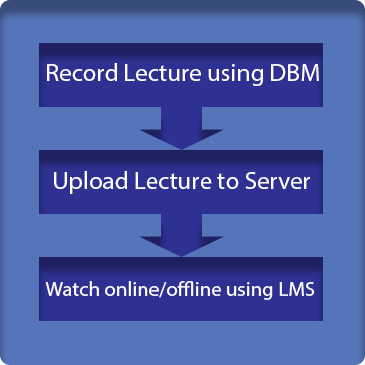
\includegraphics[width=7cm, height=6cm]{General Model}
  \caption{General Methodology View of the System}
\end{figure}


\section{General Flow}
The system consists on several modules and deliverables one of which is controller application. This application is quite important because it include major functionalities and complex image processing algorithms. Furthermore, the instructor in mainly connected to the controller application so that he/she is controlling the recording of lecture i.e. he can start, pause or stop the recording. After the lecture is recorded, he can replay the lecture for any further changes. When the lecture is finally uploaded to central computer, students can play lecture online or save the lecture file in .dbm(file extension) extension to watch later.\\ Offline player is also one of the major modules of the project. It plays the downloaded lecture file just like video player. Learning management system is the online platform where all uploaded online lecture hierarchy is accessible. It is a comprehensive management system designed by placing the convenience of instructor and student in focus. Reliability, security and quality are the top priorities.
A simple visual of the working of system can be seen below
\bigskip
\bigskip

\begin{figure}[h]
  \centering
  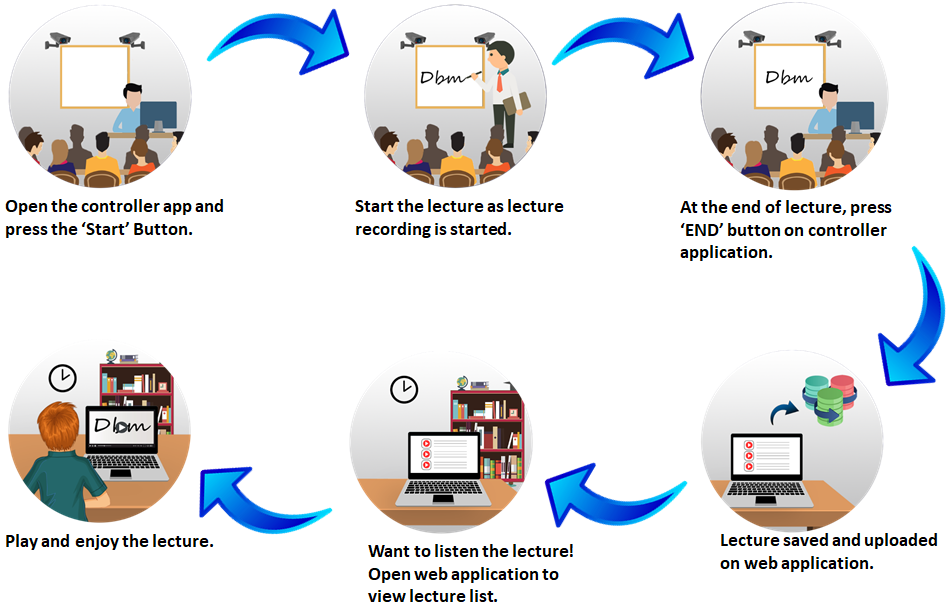
\includegraphics[width=15cm, height=11cm]{Workflow}
  \caption{General Flow of the Project}
\end{figure}
\bigskip

\section{Formulas Used}
\begin{longtable}{|>{\raggedright\arraybackslash}p{3cm}|p{4cm}|p{7cm}|}
\hline
\textbf{Descriptor} & \textbf{Explanation} & \textbf{Formula}\\
\hline
% Row 1 start
\vspace{0pt}\large Euler Angles Rotation Matrices &
Transpose of the fixed-axis matrix. Used in orientation extraction of Board Marker & 
\begin{minipage}{.3\textwidth}
      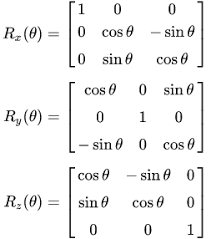
\includegraphics[width=\linewidth, height=60mm, valign=T]{EulerAngles}
\end{minipage}
\\
% Row 1 end
\hline

% Row 1 start
\vspace{0pt}\large Quaternion to Euler conversion &
Used in Marker calibration when an offset is given in particular dimension. & 
\begin{minipage}{.3\textwidth}
      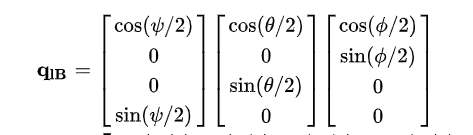
\includegraphics[width=70mm, height=30mm]{Quaternion to Euler conversion}
\end{minipage}
\\
% Row 1 end
\hline



% Row 1 start
\vspace{0pt}\large Euclidean distance formula &
Used to compute the distance in one-dimension. & 
\begin{minipage}{.3\textwidth}
      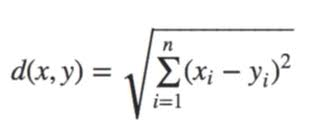
\includegraphics[width=70mm, height=40mm]{Euclidean distance formula}
\end{minipage}
\\
% Row 1 end
\hline


% Row 1 start
\vspace{0pt}\large Equation of line in slope-intercept form &
Used to draw lines and get relative position of Marker with respect to cameras. & 
\bigskip

\begin{minipage}{.3\textwidth}
      
\includegraphics[width=60mm, height=10mm]{slope-intercept form}
\end{minipage}
\\
% Row 1 end
\hline



\caption{Formulae and Equations used}
\end{longtable}

\newpage
\section{Use-Case Diagrams}
To describe the system requirements, use-case diagrams in form of simple user interaction are detailed below
\subsection{Controller Application}
The main end user of controller application is the class instructor or teacher. Teacher use the controller application in
\begin{itemize}

\item Calibrating hardware
\item Record the Lecture
\item Live Stream Lecture
\item Generate Lecture File and annotate it
\item Send Lecture file to Central Server


\end{itemize}

\begin{figure}[h]
  \centering
  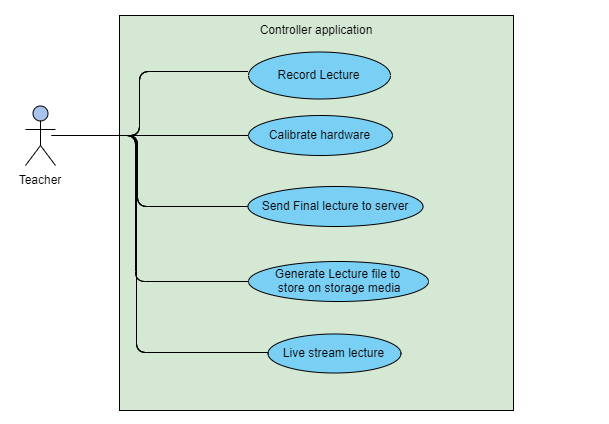
\includegraphics[width=11cm, height=10cm]{ControllerApplication}
  \caption{Use-case Diagram of Controller Application}
\end{figure}

\newpage

\subsection{Player Application}
Just like media player, the player application plays the lecture. Common end user of Player Application is student. Teacher and Student are end users of controller application. Typical actions of Player application are:

\begin{itemize}

\item View Playlist
\item Play Lecture
\item Live Stream Lecture


\end{itemize}

\bigskip

\begin{figure}[h]
  \centering
  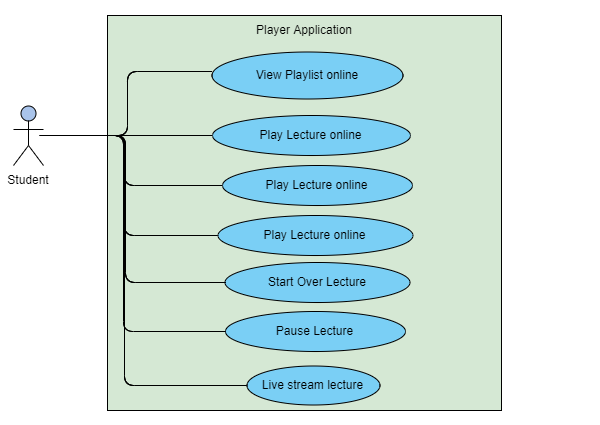
\includegraphics[width=13cm, height=14cm]{PlayerApplication}
  \caption{Use-case Diagram of Player Application}
\end{figure}

\newpage
\subsection{LMS Web Application}
LMS application is major module in terms of accessibility. Students, Teachers and administration can have access to this module simultaneously. LMS functionality is sub-divided into following different users:

\begin{itemize}

\item Admin, who manages the institute.
\item Teacher, who manages students
\item Users, who are students


\end{itemize}

\bigskip

\begin{figure}[h]
  \centering
  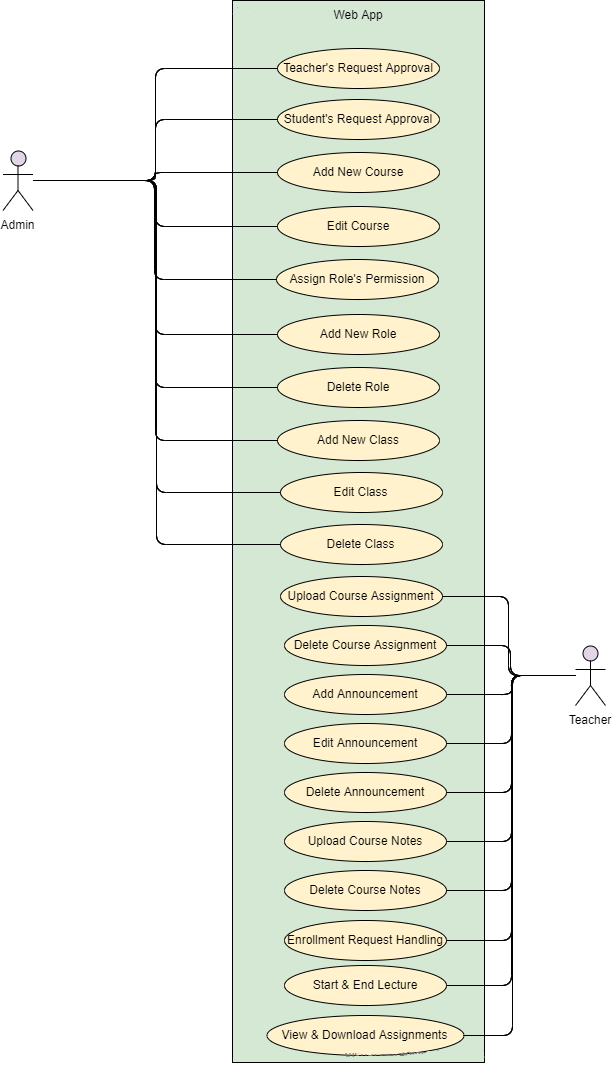
\includegraphics[width=15cm, height=14cm]{DBMUseCaseWebAppPart1}
  \caption{Use-case Diagram of LMS Web Application Part-I}
\end{figure}

\begin{figure}[h]
  \centering
  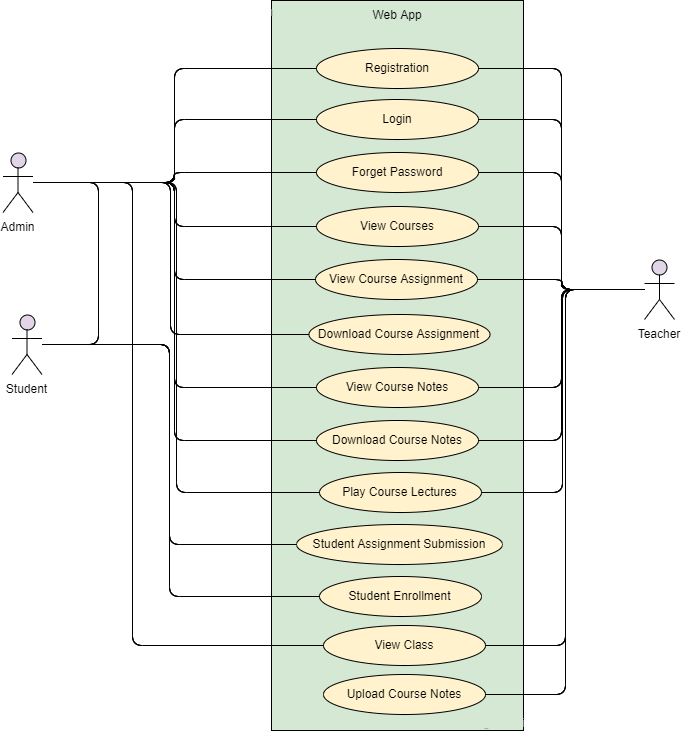
\includegraphics[width=15cm, height=14cm]{DBMUseCaseWebAppPart2}
  \caption{Use-case Diagram of LMS Web Application Part-II}
\end{figure}

\bigskip
\bigskip

\section{Use Cases(Web App)}
\subsection{Use Case UC-1: User Registration}
\textbf{Stakeholders: } University, Educational Institutes \\
\textbf{Primary Actors: } Student, Teacher \\
\textbf{Post Condition: }\\
User data successfully sent to admin request approval page.\\
\textbf{Main Success Scenario: }
\begin{enumerate}
\item User wants to register.
\item User clicks on the Register link from the main Page header.
\item Registration page will be open by the system.
\item User will enter First Name, Last Name, Email, CNIC, Password and Date of birth.
\item User will select Institute name from the select list.
\item User select whether he is teacher or a student from the select list.
\item If user is student then system will show a input box for student registration No.
\item Student will enter his registration Number.
\item User clicks the \textbf{Sign Up} button.
\item System then send data to the Admin Request Approval page for the student request approval. 
\end{enumerate}
\textbf{Alternative Flow: }\\
\\
*a. At any time system fails.
\begin{enumerate}
\item User must check the internet connectivity.
\item Restart the browser and try again.
\item Try after sometime might be servers are down.
\end{enumerate}
3a. Registration page is not opened.
\begin{enumerate}
\item Refresh the browser.
\item Reload the page and try again.
\end{enumerate}
4a. User entered the invalid First Name, Last Name.
\begin{enumerate}
\item System will show the error message.
\item System will ask the user to enter the data again.
\end{enumerate}
4b. User entered the invalid Email.
\begin{enumerate}
\item System will show the error message.
\item System will ask the user to enter the data again.
\end{enumerate}
4c. User entered the invalid CNIC.
\begin{enumerate}
\item System will show the error message.
\item System will ask the user to enter the data again.
\end{enumerate}
4d. User entered the invalid Registration No.
\begin{enumerate}
\item System will show the error message.
\item System will ask the user to enter the data again.
\end{enumerate}
4e. User entered the invalid Date of birth.
\begin{enumerate}
\item System will show the error message.
\item System will ask the user to enter the data again.
\end{enumerate}
8a. Student entered the registration No. in invalid format.
\begin{enumerate}
\item System will show the error message.
\item System will ask the user to enter the data again.
\end{enumerate}
9a. Required fields are empty.
\begin{enumerate}
\item System will show the error message.
\item System will ask the user to complete all the required fields.
\end{enumerate}
9b. Sign Up button is not clicked.
\begin{enumerate}
\item information will be saved as a draft for later use.
\end{enumerate}
\textbf{Frequency of Occurrence:}\\
One time per user.



\subsection{Use Case UC-2: User Login}
\textbf{Stakeholders: } University, Educational Institutes \\
\textbf{Primary Actors: } Student, Teacher, Admin \\
\textbf{Preconditions: }
\begin{itemize}
\item User is approved by the admin.
\item User is identified and authenticated.
\item User's record is saved.
\end{itemize}
\textbf{Post Condition: }
\begin{itemize}
\item User is logged in into the system.
\item User has access to different functionality of the system.
\end{itemize}

\textbf{Main Success Scenario:}
\begin{enumerate}
\item User wants to login.
\item User clicked on the login link to access the login page from the header.
\item System open the login page for the user.
\item User enter email address along with the password.
\item User clicked the \textbf{Sign In} button.
\item System validates the user email and password.
\item System will redirect the user to next page.
\end{enumerate}
\textbf{Alternative Flows:}\\
\\
*a. At any time, system fails.
\begin{enumerate}
\item User must check the internet connectivity.
\item Restart the browser and try again.
\item Try after sometime might be servers are down.
\end{enumerate}
3a. Login page is not opened.
\begin{enumerate}
\item Refresh the browser.
\item Reload the page and try again.
\end{enumerate}
4a. User entered invalid email and password.
\begin{enumerate}
\item System will show the error message.
\item System will ask the user to enter the data again.
\end{enumerate}
5a. Required fields are empty.
\begin{enumerate}
\item System will show the error message.
\item System will ask the user to complete all the required fields.
\end{enumerate}
6a. User is not identified or authenticated.
\begin{enumerate}
\item System will show error message.
\item System will ask the user to register yourself first.
\end{enumerate}
\textbf{Frequency of Occurrence:}\\
Whenever the user wants to login.





\subsection{Use Case UC-3: Teacher's Requests Approval/Disapproval}
\textbf{Stakeholders: } University, Educational Institutes \\
\textbf{Primary Actors: } Admin \\
\textbf{Preconditions:}
\begin{itemize}
\item Admin is logged in the system..
\item Admin is identified and authenticated.
\end{itemize}
\textbf{Post Conditions: }
\begin{itemize}
\item Requests are approved / disapproved.
\item On approval / disapproval, Email is sent to the teacher.
\item Teachers can login to the system.
\end{itemize}
\textbf{Main Success Scenario:}
\begin{enumerate}
\item Admin wants to handle the requests of teachers.
\item Admin clicks on the Teacher requests approval link from the header.
\item System open the \textbf{teachers request approval} page for the admin.
\item Admin can see the list of all the requests of teachers.
\item Admin clicks on the \textbf{Approve} button for approval of request.
\item System send the approval email to that teacher.
\item System show the success message to admin that email is sent.
\item System saves the record of the teacher.
\item System removes the request from the page.
\item Admin disapprove the request of a teacher by clicking on \textbf{Disapprove} button.
\item System delete that temporary record of the user.
\item System send an disapproval email to the teacher.
\item System show the success message to admin that email is sent.
\item System removes the request from the page.
\end{enumerate}
\textbf{Alternative Flows:}\\
\\
*a. At any time, system fails.
\begin{enumerate}
\item User must check the internet connectivity.
\item Restart the browser and try again.
\item Try after sometime might be servers are down.
\end{enumerate}
3a. Page is not opened.
\begin{enumerate}
\item Refresh the browser.
\item Reload the page and try again.
\end{enumerate}
5a. Approve button is not working properly.
\begin{enumerate}
\item Admin must have to refresh the page.
\item Restart the browser and try again.
\item May be some backend issue, resolve that issue.
\end{enumerate}
6-7a. Email is not sent to the teacher.
\begin{enumerate}
\item Admin must again approve the request of teacher.
\item May be some backend issue, resolve that issue.
\end{enumerate}
8-9a. Request is not removed from the page and record is unsaved.
\begin{enumerate}
\item Admin must again approve the request of teacher.
\item May be some backend issue, resolve that issue.
\end{enumerate}
10a. Disapprove button is not working properly.
\begin{enumerate}
\item Admin must have to refresh the page.
\item Restart the browser and try again.
\item May be some backend issue, resolve that issue.
\end{enumerate}
12-13a. Email is not sent to the teacher.
\begin{enumerate}
\item Admin must again approve the request of teacher.
\item May be some backend issue, resolve that issue.
\end{enumerate}
14a. Request is not removed from the page.
\begin{enumerate}
\item Admin must again approve the request of teacher.
\item May be some backend issue, resolve that issue.
\end{enumerate}
\textbf{Frequency of Occurrence:}\\
Whenever the requests appear on the page.
\\
\textbf{Open Issues:}\\
What will happen if admin has mistakenly approve or disapprove the request of teacher?


\subsection{Use Case UC-4: Student's Requests Approval/Disapprovals}
\textbf{Stakeholders: } University, Educational Institutes \\
\textbf{Primary Actors: } Admin \\
\textbf{Preconditions:}
\begin{itemize}
\item Admin is logged in the system..
\item Admin is identified and authenticated.
\end{itemize}
\textbf{Post Conditions: }
\begin{itemize}
\item Requests are approved / disapproved.
\item On approval / disapproval, Email is sent to the student.
\item Students can login to the system.
\end{itemize}
\textbf{Main Success Scenario:}
\begin{enumerate}
\item Admin wants to handle the requests of students.
\item Admin clicks on the student requests approval link from the header.
\item System open the \textbf{Students Request Approval} page for the admin.
\item Admin can see the list of all the request of students.
\item Admin clicks on the \textbf{Approve} button for approval of request.
\item System send the approval email to that student.
\item System show the success message to admin that email is sent.
\item System saves the record of the student.
\item System removes the request from the page.
\item Admin disapprove the request of a student by clicking on \textbf{disapprove} button.
\item System delete that temporary record of the user.
\item System send an disapproval email to the student.
\item System show the success message to admin that email is sent.
\item System removes the request from the page.
\end{enumerate}
\textbf{Alternative Flows:}\\
\\
*a. At any time, system fails.
\begin{enumerate}
\item User must check the internet connectivity.
\item Restart the browser and try again.
\item Try after sometime might be servers are down.
\end{enumerate}
3a. Page is not opened.
\begin{enumerate}
\item Refresh the browser.
\item Reload the page and try again.
\end{enumerate}
5a. Approve button is not working properly.
\begin{enumerate}
\item Admin must have to refresh the page.
\item Restart the browser and try again.
\item May be some backend issue, resolve that issue.
\end{enumerate}
6-7a. Email is not sent to the student.
\begin{enumerate}
\item Admin must again approve the request of student.
\item May be some backend issue, resolve that issue.
\end{enumerate}
8-9a. Request is not removed from the page and record is unsaved.
\begin{enumerate}
\item Admin must again approve the request of student.
\item May be some backend issue, resolve that issue.
\end{enumerate}
10a. Disapprove button is not working properly.
\begin{enumerate}
\item Admin must have to refresh the page.
\item Restart the browser and try again.
\item May be some backend issue, resolve that issue.
\end{enumerate}
12-13a. Email is not sent to the teacher.
\begin{enumerate}
\item Admin must again approve the request of student.
\item May be some backend issue, resolve that issue.
\end{enumerate}
14a. Request is not removed from the page.
\begin{enumerate}
\item Admin must again approve the request of student.
\item May be some backend issue, resolve that issue.
\end{enumerate}
\textbf{Frequency of Occurrence:}\\
Whenever the admin get requests from students.
\\
\textbf{Open Issues:}\\
What will happen if admin has mistakenly approve or disapprove the request of student?


\subsection{Use Case UC-5: Add New Course}
\textbf{Stakeholders: } University, Educational Institutes \\
\textbf{Primary Actors: } Admin \\
\textbf{Preconditions:}
\begin{itemize}
\item Admin is logged in the system.
\item Admin is identified and authenticated.
\end{itemize}
\textbf{Post Condition: }\\
Course is added successfully.\\
\textbf{Main Success Scenario:}
\begin{enumerate}
\item Admin want to add new course.
\item He clicks on the course link from the header.
\item All courses screen will be open.
\item Admin clicks the \textbf{Add Course} button to add new course.
\item System open a new page.
\item Admin add all course related information.
\item Admin clicks the \textbf{Submit} button. 
\end{enumerate}
\textbf{Alternative Flows:}\\
*a. At any time, System fails.
\begin{enumerate}
\item User must check the internet connectivity.
\item Restart the browser and try again.
\item Try after sometime might be servers are down.
\end{enumerate}
2a. Courses link is not shown on the header.
\begin{enumerate}
\item Admin must have to refresh the page.
\item Restart the browser and try again.
\end{enumerate} 
3a. All courses page is not opened.
\begin{enumerate}
\item Admin must check the internet connectivity.
\item Refresh the browser.
\item Reload the page and try again.
\end{enumerate}
4a. Add button not working.
\begin{enumerate}
\item Admin must check the internet connectivity.
\item Refresh the browser.
\item Reload the page and try again.
\item May be some backend issue, try to resolve that issue.
\end{enumerate}
5a. New page is not appearing.
\begin{enumerate}
\item Admin must check the internet connectivity.
\item Refresh the browser.
\item Try for sometime, may be servers are down.
\end{enumerate}
6a. Admin enter invalid data.
\begin{enumerate}
\item System will prompt an error message.
\item System will ask the user to enter valid data.
\end{enumerate}
7a. Required fields are empty.
\begin{enumerate}
\item System will prompt an error message.
\item System will ask the user to enter all the required information.
\end{enumerate}
7b. Admin don't click on \textbf{Add} button.
\begin{enumerate}
\item System will save the record as draft for later use.
\end{enumerate}
\textbf{Frequency of Occurrence:}\\
Whenever the admin wants to add new course.



\subsection{Use Case UC-6: Edit Course}
\textbf{Stakeholders: } University, Educational Institutes \\
\textbf{Primary Actors: } Admin \\
\textbf{Preconditions:}
\begin{itemize}
\item Admin is logged in the system.
\item Admin is identified and authenticated.
\item Course must be added.
\end{itemize}
\textbf{Post Condition: }\\
Course is updated successfully.\\

\textbf{Main Success Scenario:}
\begin{enumerate}
\item Admin wants to edit particular course.
\item Admin clicks on the courses link from the header.
\item System open a page of all courses.
\item Admin click on the \textbf{Edit} button of course which he wants to update.
\item Course Edit screen will appear.
\item Admin update the required information.
\item Admin clicks the \textbf{Update Course} button.
\item System update the course.
\end{enumerate}
\textbf{Alternative Flows:}\\
\\
*a. At any time, System fails.
\begin{enumerate}
\item User must check the internet connectivity.
\item Restart the browser and try again.
\item Try after sometime might be servers are down.
\end{enumerate}
2a. Courses link is not shown on the header.
\begin{enumerate}
\item Admin must have to refresh the page.
\item Restart the browser and try again.
\end{enumerate} 
3a. All courses page is not opened.
\begin{enumerate}
\item Admin must check the internet connectivity.
\item Refresh the browser.
\item Reload the page and try again.
\end{enumerate}
4a. Edit button not working.
\begin{enumerate}
\item Admin must check the internet connectivity.
\item Refresh the browser.
\item Reload the page and try again.
\item May be some backend issue, try to resolve that issue.
\end{enumerate}
5a. Edit Course page is not appearing.
\begin{enumerate}
\item Admin must check the internet connectivity.
\item Refresh the browser.
\item Try for sometime, may be servers are down.
\end{enumerate}
6a. Admin enter invalid data.
\begin{enumerate}
\item System will prompt an error message.
\item System will ask the user to enter valid data.
\end{enumerate}
7a. Required fields are empty.
\begin{enumerate}
\item System will prompt an error message.
\item System will ask the user to enter all the required information.
\end{enumerate}
7b. Admin don't click on \textbf{Update Course} button.
\begin{enumerate}
\item System will save the record as draft for later use.
\end{enumerate}
\textbf{Frequency of Occurrence:}\\
Whenever the user wants to update the course information.



\subsection{Use Case UC-7: Delete Course}
\textbf{Stakeholders: } University, Educational Institutes \\
\textbf{Primary Actors: } Admin \\
\textbf{Preconditions:}
\begin{itemize}
\item Admin is logged in the system.
\item Admin is identified and authenticated.
\item Course must be added.
\end{itemize}
\textbf{Post Condition: }\\
Course is deleted successfully.\\
\textbf{Main Success Scenario:}
\begin{enumerate}
\item Admin wants to delete particular course.
\item Admin clicks on the courses link from the header.
\item System open a page of all courses.
\item Admin click on the \textbf{Delete} button of course which he wants to delete.
\item A pop message show "Are you sure you want to delete the course?".
\item Admin clicks the sure button.
\item System delete that course from the record.
\end{enumerate}
\textbf{Alternative Flows:}\\
\\
*a. At any time, System fails.
\begin{enumerate}
\item User must check the internet connectivity.
\item Restart the browser and try again.
\item Try after sometime might be servers are down.
\end{enumerate}
2a. Courses link is not shown on the header.
\begin{enumerate}
\item Admin must have to refresh the page.
\item Restart the browser and try again.
\end{enumerate} 
3a. All courses page is not opened.
\begin{enumerate}
\item Admin must check the internet connectivity.
\item Refresh the browser.
\item Reload the page and try again.
\end{enumerate}
4a. Delete button not working.
\begin{enumerate}
\item Admin must check the internet connectivity.
\item Refresh the browser.
\item Reload the page and try again.
\item May be some backend issue, try to resolve that issue.
\end{enumerate}
5a. Admin clicks the sure button but course is not deleted.
\begin{enumerate}
\item May be servers are down. Try again after sometime.
\item Press again the delete button.
\end{enumerate}
\textbf{Frequency of Occurrence:}\\
Whenever the admin wants to delete a course.
\textbf{Open Issues:}\\
What will happen if admin has mistakenly deleted the course?



\subsection{Use Case UC-8: View Courses}
\textbf{Stakeholders: } University, Educational Institutes \\
\textbf{Primary Actors: }Admin,Teacher, Student \\
\textbf{Preconditions:}
\begin{itemize}
\item User is logged in the system.
\item User is identified and authenticated.
\item Courses must be added.
\end{itemize}
\textbf{Post Condition: }\\
Courses List is viewed successfully.\\
\textbf{Main Success Scenario:}
\begin{enumerate}
\item Admin wants to view all courses.
\item Admin clicks on the courses link from the header.
\item System open a page of all courses.
\end{enumerate}
\textbf{Alternative Flows:}\\
\\
*a. At any time, System fails.
\begin{enumerate}
\item User must check the internet connectivity.
\item Restart the browser and try again.
\item Try after sometime might be servers are down.
\end{enumerate}
2a. Courses link is not shown on the header.
\begin{enumerate}
\item Admin must have to refresh the page.
\item Restart the browser and try again.
\end{enumerate} 
3a. All courses page is not opened.
\begin{enumerate}
\item Admin must check the internet connectivity.
\item Refresh the browser.
\item Reload the page and try again.
\end{enumerate}
\textbf{Frequency of Occurrence:}\\
Whenever the user wants to view all course.




\subsection{Use Case UC-9: Upload Course Assignment}
\textbf{Stakeholders: } University, Educational Institutes \\
\textbf{Primary Actors: }Teacher \\
\textbf{Preconditions:}
\begin{itemize}
\item Teacher is logged in the system.
\item User is identified and authenticated.
\item Course is assigned to the teacher.
\end{itemize}
\textbf{Post Condition: }\\
Course assignment is uploaded successfully.\\
\textbf{Main Success Scenario:}
\begin{enumerate}
\item Teacher wants to upload course assignment.
\item Teacher clicks on the courses link from the header.
\item System opens a page of all courses.
\item Teacher clicks on the \textbf{View} button of course of which he wants to upload assignment.
\item System opens a course dashboard page.
\item Teacher clicks on the \textbf{Assignments} tab.
\item System opens the assignments page.
\item Teacher click on \textbf{Upload Assignment} button.
\item System opens upload assignment page.
\item Teacher enters all the data.
\item System validates the data.
\item Teacher press the \textbf{Upload Assignment} button.
\item System saves the assignment record.
\end{enumerate}
\textbf{Alternative Flows:}\\
\\
*a. At any time, System fails.
\begin{enumerate}
\item User must check the internet connectivity.
\item Restart the browser and try again.
\item Try after sometime might be servers are down.
\end{enumerate}
2a. Courses link is not shown on the header.
\begin{enumerate}
\item User must have to refresh the page.
\item Restart the browser and try again.
\end{enumerate} 
3a. All courses page is not opened.
\begin{enumerate}
\item User must check the internet connectivity.
\item Refresh the browser.
\item Reload the page and try again.
\end{enumerate}
4a. View button not working.
\begin{enumerate}
\item User must check the internet connectivity.
\item Refresh the browser.
\item Reload the page and try again.
\item May be some backend issue, try to resolve that issue.
\end{enumerate}
5a. Course dasboard page is not opened.
\begin{enumerate}
\item User must check the internet connectivity.
\item Refresh the browser.
\item Reload the page and try again.
\end{enumerate}
6a. Assignments tab not working.
\begin{enumerate}
\item Reload the page and try again.
\item May be some backend issue, try to resolve that issue.
\end{enumerate}
7a. Assignments page is not opened.
\begin{enumerate}
\item User must check the internet connectivity.
\item Refresh the browser.
\item Reload the page and try again.
\end{enumerate}
8a. Upload assignment button not working.
\begin{enumerate}
\item Reload the page and try again.
\item Check the internet connectivity.
\item May be some backend issue, try to resolve that issue.
\end{enumerate}
9a. Upload assignment page is not opened.
\begin{enumerate}
\item User must check the internet connectivity.
\item Refresh the browser.
\item Reload the page and try again.
\end{enumerate}
10-11a. User enter invalid data.
\begin{enumerate}
\item System will show error message.
\item System will ask the user to enter the data again.
\end{enumerate}
12a. Required fields are empty.
\begin{enumerate}
\item System will show error message.
\item System will ask the user to enter the required data. 
\end{enumerate}
\textbf{Frequency of Occurrence:}\\
Whenever user wants to upload assignments.



\subsection{Use Case UC-10: View Course Assignments}
\textbf{Stakeholders: } University, Educational Institutes \\
\textbf{Primary Actors: }Teacher, Student \\
\textbf{Preconditions:}
\begin{itemize}
\item User is identified and authenticated.
\item User is logged in the system.
\item Student is enrolled in that course.
\item Course is assigned to teacher.
\end{itemize}
\textbf{Post Condition: }\\
Course Assignment viewed successfully.\\
\textbf{Main Success Scenario:}
\begin{enumerate}
\item User wants to view course assignment.
\item User clicks on the courses link from the header.
\item System opens a page of all courses.
\item User clicks on the \textbf{View} button of course of which he wants to view assignment.
\item System opens a course dashboard page.
\item User clicks on the \textbf{Assignments} tab.
\item System opens the assignments page.
\end{enumerate}
\textbf{Alternative Flows:}\\
\\
*a. At any time, System fails.
\begin{enumerate}
\item User must check the internet connectivity.
\item Restart the browser and try again.
\item Try after sometime might be servers are down.
\end{enumerate}
2a. Courses link is not shown on the header.
\begin{enumerate}
\item User must have to refresh the page.
\item Restart the browser and try again.
\end{enumerate} 
3a. All courses page is not opened.
\begin{enumerate}
\item User must check the internet connectivity.
\item Refresh the browser.
\item Reload the page and try again.
\end{enumerate}
4a. View button not working.
\begin{enumerate}
\item User must check the internet connectivity.
\item Refresh the browser.
\item Reload the page and try again.
\item May be some backend issue, try to resolve that issue.
\end{enumerate}
5a. Course dasboard page is not opened.
\begin{enumerate}
\item User must check the internet connectivity.
\item Refresh the browser.
\item Reload the page and try again.
\end{enumerate}
6a. Assignments tab not working.
\begin{enumerate}
\item Reload the page and try again.
\item May be some backend issue, try to resolve that issue.
\end{enumerate}
7a. Assignments page is not opened.
\begin{enumerate}
\item User must check the internet connectivity.
\item Refresh the browser.
\item Reload the page and try again.
\end{enumerate}
\textbf{Frequency of Occurrence:}\\
Whenever user wants to view assignments.



\subsection{Use Case UC-11: Download Course Assignment}
\textbf{Stakeholders: } University, Educational Institutes \\
\textbf{Primary Actors: }Teacher, Student \\
\textbf{Preconditions:}
\begin{itemize}
\item User is logged in the system.
\item User is identified and authenticated.
\item Course is assigned to the teacher.
\item Student is enrolled in that course.
\end{itemize}
\textbf{Post Condition: }\\
Course assignment is downloaded successfully.\\
\textbf{Main Success Scenario:}
\begin{enumerate}
\item User wants to download course assignment.
\item User clicks on the courses link from the header.
\item System opens a page of all courses.
\item User clicks on the \textbf{View} button of course of which he wants to download assignment.
\item System opens a course dashboard page.
\item User clicks on the \textbf{Assignments} tab.
\item System opens the assignments page.
\item User click on \textbf{Download Assignment} button.
\item System downloads the assignment file for the user.
\end{enumerate}
\textbf{Alternative Flows:}\\
\\
*a. At any time, System fails.
\begin{enumerate}
\item User must check the internet connectivity.
\item Restart the browser and try again.
\item Try after sometime might be servers are down.
\end{enumerate}
2a. Courses link is not shown on the header.
\begin{enumerate}
\item User must have to refresh the page.
\item Restart the browser and try again.
\end{enumerate} 
3a. All courses page is not opened.
\begin{enumerate}
\item User must check the internet connectivity.
\item Refresh the browser.
\item Reload the page and try again.
\end{enumerate}
4a. View button not working.
\begin{enumerate}
\item User must check the internet connectivity.
\item Refresh the browser.
\item Reload the page and try again.
\item May be some backend issue, try to resolve that issue.
\end{enumerate}
5a. Course dasboard page is not opened.
\begin{enumerate}
\item User must check the internet connectivity.
\item Refresh the browser.
\item Reload the page and try again.
\end{enumerate}
6a. Assignments tab not working.
\begin{enumerate}
\item Reload the page and try again.
\item May be some backend issue, try to resolve that issue.
\end{enumerate}
7a. Assignments page is not opened.
\begin{enumerate}
\item User must check the internet connectivity.
\item Refresh the browser.
\item Reload the page and try again.
\end{enumerate}
8a. Download assignment button not working.
\begin{enumerate}
\item Reload the page and try again.
\item Check the internet connectivity.
\item May be some backend issue, try to resolve that issue.
\end{enumerate}
\textbf{Frequency of Occurrence:}\\
Whenever user wants to download assignments.



\subsection{Use Case UC-12: Delete Course Assignment}
\textbf{Stakeholders: } University, Educational Institutes \\
\textbf{Primary Actors: }Teacher \\
\textbf{Preconditions:}
\begin{itemize}
\item Teacher is logged in the system.
\item User is identified and authenticated.
\item Course is assigned to the teacher.
\end{itemize}
\textbf{Post Condition: }\\
Course assignment is deleted successfully.\\
\textbf{Main Success Scenario:}
\begin{enumerate}
\item Teacher wants to delete course assignment.
\item Teacher clicks on the courses link from the header.
\item System opens a page of all courses.
\item Teacher clicks on the \textbf{View} button of course of which he wants to upload assignment.
\item System opens a course dashboard page.
\item Teacher clicks on the \textbf{Assignments} tab.
\item System opens the assignments page.
\item Teacher click on \textbf{Delete Assignment} button.
\item A pop message show "Are you sure you want to delete the assignment?".
\item Teacher clicks the sure button.
\item System delete that assignment from the record.
\end{enumerate}
\textbf{Alternative Flows:}\\
\\
*a. At any time, System fails.
\begin{enumerate}
\item User must check the internet connectivity.
\item Restart the browser and try again.
\item Try after sometime might be servers are down.
\end{enumerate}
2a. Courses link is not shown on the header.
\begin{enumerate}
\item User must have to refresh the page.
\item Restart the browser and try again.
\end{enumerate} 
3a. All courses page is not opened.
\begin{enumerate}
\item User must check the internet connectivity.
\item Refresh the browser.
\item Reload the page and try again.
\end{enumerate}
4a. View button not working.
\begin{enumerate}
\item User must check the internet connectivity.
\item Refresh the browser.
\item Reload the page and try again.
\item May be some backend issue, try to resolve that issue.
\end{enumerate}
5a. Course dasboard page is not opened.
\begin{enumerate}
\item User must check the internet connectivity.
\item Refresh the browser.
\item Reload the page and try again.
\end{enumerate}
6a. Assignments tab not working.
\begin{enumerate}
\item Reload the page and try again.
\item May be some backend issue, try to resolve that issue.
\end{enumerate}
7a. Assignments page is not opened.
\begin{enumerate}
\item User must check the internet connectivity.
\item Refresh the browser.
\item Reload the page and try again.
\end{enumerate}
8a. Delete assignment button not working.
\begin{enumerate}
\item Reload the page and try again.
\item May be some backend issue, try to resolve that issue.
\end{enumerate}
10-11a. Teacher clicks the sure button but assignment is not deleted.
\begin{enumerate}
\item May be servers are down. Try again after sometime.
\item Press again the delete button.
\end{enumerate}
\textbf{Frequency of Occurrence:}\\
Whenever user wants to delete assignment.



\subsection{Use Case UC-13: Add Course Announcement}
\textbf{Stakeholders: } University, Educational Institutes \\
\textbf{Primary Actors: }Teacher \\
\textbf{Preconditions:}
\begin{itemize}
\item Teacher is logged in the system.
\item Teacher is identified and authenticated.
\item Course is assigned to the teacher.
\end{itemize}
\textbf{Post Condition: }\\
Course Announcement is added successfully.\\
\\
\textbf{Main Success Scenario:}
\begin{enumerate}
\item Teacher wants to add course related announcement.
\item Teacher clicks on the courses link from the header.
\item System opens a page of all courses.
\item Teacher clicks on the \textbf{View} button of course of which he wants to add announcement.
\item System opens a course dashboard page.
\item Teacher clicks on the \textbf{Announcement} tab.
\item System opens the announcement page.
\item Teacher click on \textbf{Add Announcement} button.
\item System opens add announcement page.
\item Teacher enters all the data.
\item System validates the data.
\item Teacher press the \textbf{Add Announcement} button.
\item System saves the announcement record.
\end{enumerate}
\textbf{Alternative Flows:}\\
\\
*a. At any time, System fails.
\begin{enumerate}
\item User must check the internet connectivity.
\item Restart the browser and try again.
\item Try after sometime might be servers are down.
\end{enumerate}
2a. Courses link is not shown on the header.
\begin{enumerate}
\item User must have to refresh the page.
\item Restart the browser and try again.
\end{enumerate} 
3a. All courses page is not opened.
\begin{enumerate}
\item User must check the internet connectivity.
\item Refresh the browser.
\item Reload the page and try again.
\end{enumerate}
4a. View button not working.
\begin{enumerate}
\item User must check the internet connectivity.
\item Refresh the browser.
\item Reload the page and try again.
\item May be some backend issue, try to resolve that issue.
\end{enumerate}
5a. Course dasboard page is not opened.
\begin{enumerate}
\item User must check the internet connectivity.
\item Refresh the browser.
\item Reload the page and try again.
\end{enumerate}
6a. Announcement tab not working.
\begin{enumerate}
\item Reload the page and try again.
\item May be some backend issue, try to resolve that issue.
\end{enumerate}
7a. Announcement page is not opened.
\begin{enumerate}
\item User must check the internet connectivity.
\item Refresh the browser.
\item Reload the page and try again.
\end{enumerate}
8a. Add announcement button not working.
\begin{enumerate}
\item Reload the page and try again.
\item May be some backend issue, try to resolve that issue.
\end{enumerate}
9a. Add announcement page is not opened.
\begin{enumerate}
\item User must check the internet connectivity.
\item Refresh the browser.
\item Reload the page and try again.
\end{enumerate}
\textbf{Frequency of Occurrence:}\\
Whenever user wants to add announcement.



\subsection{Use Case UC-14 :Edit Course Announcement}
\textbf{Stakeholders: } University, Educational Institutes \\
\textbf{Primary Actors: }Teacher \\
\textbf{Preconditions:}
\begin{itemize}
\item Teacher is identified and authenticated.
\item Teacher is logged in the system.
\item Course is assigned to the teacher.
\end{itemize}
\textbf{Post Condition: }\\
Course Announcement is updated successfully.\\

\textbf{Main Success Scenario:}
\begin{enumerate}
\item Teacher wants to edit course related announcement.
\item Teacher clicks on the courses link from the header.
\item System opens a page of all courses.
\item Teacher clicks on the \textbf{View} button of course of which he wants to edit announcement.
\item System opens a course dashboard page.
\item Teacher clicks on the \textbf{Announcement} tab.
\item System opens the announcement page.
\item Teacher click on \textbf{Edit Announcement} button of the announcement.
\item System opens edit announcement page.
\item Teacher edit the required data.
\item System validates the data.
\item Teacher press the \textbf{Update Announcement} button.
\item System updates the announcement record.
\end{enumerate}
\textbf{Alternative Flows:}\\
\\
*a. At any time, System fails.
\begin{enumerate}
\item User must check the internet connectivity.
\item Restart the browser and try again.
\item Try after sometime might be servers are down.
\end{enumerate}
2a. Courses link is not shown on the header.
\begin{enumerate}
\item User must have to refresh the page.
\item Restart the browser and try again.
\end{enumerate} 
3a. All courses page is not opened.
\begin{enumerate}
\item User must check the internet connectivity.
\item Refresh the browser.
\item Reload the page and try again.
\end{enumerate}
4a. View button not working.
\begin{enumerate}
\item User must check the internet connectivity.
\item Refresh the browser.
\item Reload the page and try again.
\item May be some backend issue, try to resolve that issue.
\end{enumerate}
5a. Course dasboard page is not opened.
\begin{enumerate}
\item User must check the internet connectivity.
\item Refresh the browser.
\item Reload the page and try again.
\end{enumerate}
6a. Announcement tab not working.
\begin{enumerate}
\item Reload the page and try again.
\item May be some backend issue, try to resolve that issue.
\end{enumerate}
7a. Announcement page is not opened.
\begin{enumerate}
\item User must check the internet connectivity.
\item Refresh the browser.
\item Reload the page and try again.
\end{enumerate}
8a. Edit announcement button not working.
\begin{enumerate}
\item Reload the page and try again.
\item May be some backend issue, try to resolve that issue.
\end{enumerate}
9a. Update announcement page is not opened.
\begin{enumerate}
\item User must check the internet connectivity.
\item Refresh the browser.
\item Reload the page and try again.
\end{enumerate}
10a. Teacher enters the invalid data.
\begin{enumerate}
\item System prompts the error message.
\item System will ask the user to enter the data again.
\end{enumerate}
12a. Required fields are empty.
\begin{enumerate}
\item System prompts the error message.
\item System will ask the user to enter the data in the empty fields.
\end{enumerate}
\textbf{Frequency of Occurrence:}\\
Whenever user wants to update announcement.



\subsection{Use Case UC-15: Delete Course Announcement}
\textbf{Stakeholders: } University, Educational Institutes \\
\textbf{Primary Actors: }Teacher \\
\textbf{Preconditions:}
\begin{itemize}
\item User is identified and authenticated.
\item User is logged in the system.
\item Course is assigned to the teacher.
\end{itemize}
\textbf{Post Condition: }\\
Course announcement is deleted successfully.\\
\textbf{Main Success Scenario:}
\begin{enumerate}
\item Teacher wants to delete course announcement.
\item Teacher clicks on the courses link from the header.
\item System opens a page of all courses.
\item Teacher clicks on the \textbf{View} button of course of which he wants to delete announcement.
\item System opens a course dashboard page.
\item Teacher clicks on the \textbf{Announcements} tab.
\item System opens the announcements page.
\item Teacher click on \textbf{Delete Announcement} button.
\item A pop message show "Are you sure you want to delete the announcement?".
\item Teacher clicks the sure button.
\item System delete that announcement from the record.
\end{enumerate}
\textbf{Alternative Flows:}\\
\\
*a. At any time, System fails.
\begin{enumerate}
\item User must check the internet connectivity.
\item Restart the browser and try again.
\item Try after sometime might be servers are down.
\end{enumerate}
2a. Courses link is not shown on the header.
\begin{enumerate}
\item User must have to refresh the page.
\item Restart the browser and try again.
\end{enumerate} 
3a. All courses page is not opened.
\begin{enumerate}
\item User must check the internet connectivity.
\item Refresh the browser.
\item Reload the page and try again.
\end{enumerate}
4a. View button not working.
\begin{enumerate}
\item User must check the internet connectivity.
\item Refresh the browser.
\item Reload the page and try again.
\item May be some backend issue, try to resolve that issue.
\end{enumerate}
5a. Course dasboard page is not opened.
\begin{enumerate}
\item User must check the internet connectivity.
\item Refresh the browser.
\item Reload the page and try again.
\end{enumerate}
6a. Announcement tab not working.
\begin{enumerate}
\item Reload the page and try again.
\item May be some backend issue, try to resolve that issue.
\end{enumerate}
7a. Announcement page is not opened.
\begin{enumerate}
\item User must check the internet connectivity.
\item Refresh the browser.
\item Reload the page and try again.
\end{enumerate}
8a. Delete announcement button not working.
\begin{enumerate}
\item Reload the page and try again.
\item May be some backend issue, try to resolve that issue.
\end{enumerate}
10-11a. Teacher clicks the sure button but announcement is not deleted.
\begin{enumerate}
\item May be servers are down. Try again after sometime.
\item Press again the delete button.
\end{enumerate}
\textbf{Frequency of Occurrence:}\\
Whenever user wants to delete announcement.\\
\textbf{Open Issues:}\\
What will happen if teacher have mistakenly delete the announcement?



\subsection{Use Case UC-16: Student Assignment Submission}
\textbf{Stakeholders: } University, Educational Institutes \\
\textbf{Primary Actors: }Student \\
\textbf{Preconditions:}
\begin{itemize}
\item User is identified and authenticated.
\item User is logged in the system.
\item Student is enrolled in that course.
\end{itemize}
\textbf{Post Condition: }\\
Assignment is submitted successfully.\\
\\
\textbf{Main Success Scenario:}
\begin{enumerate}
\item Student wants to submit course assignment.
\item Student clicks on the courses link from the header.
\item System opens a page of all courses.
\item Student clicks on the \textbf{View} button of course of which he wants to submit assignment.
\item System opens a course dashboard page.
\item Student clicks on the \textbf{Assignment} tab.
\item System opens the assignment page.
\item Student click on \textbf{Submit Assignment} button.
\item System open a new page.
\item Student upload assignment file which he/she wants to submit.
\item Student clicks on the \textbf{Submit} button.
\item System save the assignment of student in the record.
\end{enumerate}
\textbf{Alternative Flows:}\\
\\
*a. At any time, System fails.
\begin{enumerate}
\item User must check the internet connectivity.
\item Restart the browser and try again.
\item Try after sometime might be servers are down.
\end{enumerate}
2a. Courses link is not shown on the header.
\begin{enumerate}
\item User must have to refresh the page.
\item Restart the browser and try again.
\end{enumerate} 
3a. All courses page is not opened.
\begin{enumerate}
\item User must check the internet connectivity.
\item Refresh the browser.
\item Reload the page and try again.
\end{enumerate}
4a. View button not working.
\begin{enumerate}
\item User must check the internet connectivity.
\item Refresh the browser.
\item Reload the page and try again.
\item May be some backend issue, try to resolve that issue.
\end{enumerate}
5a. Course dasboard page is not opened.
\begin{enumerate}
\item User must check the internet connectivity.
\item Refresh the browser.
\item Reload the page and try again.
\end{enumerate}
6a. Assignment tab not working.
\begin{enumerate}
\item Reload the page and try again.
\item May be some backend issue, try to resolve that issue.
\end{enumerate}
7a. Assignment page is not opened.
\begin{enumerate}
\item User must check the internet connectivity.
\item Refresh the browser.
\item Reload the page and try again.
\end{enumerate}
8a. Submit assignment button not working.
\begin{enumerate}
\item Reload the page and try again.
\item May be some backend issue, try to resolve that issue.
\end{enumerate}
9a. Submit assignment page is not opened.
\begin{enumerate}
\item User must check the internet connectivity.
\item Reload the page and try again.
\item May be some backend issue, try to resolve that issue.
\end{enumerate}
11a. Assignment file is not attached.
\begin{enumerate}
\item System will show error message.
\item System will ask the user to attach the file first.
\end{enumerate}
\textbf{Frequency of Occurrence:}\\
Whenever user wants to submit assignment.



\subsection{Use Case UC-17: Upload Course Notes}
\textbf{Stakeholders: } University, Educational Institutes \\
\textbf{Primary Actors: }Teacher \\

\textbf{Preconditions:}
\begin{itemize}
\item Teacher is logged in the system.
\item User is identified and authenticated.
\item Course is assigned to the teacher.
\end{itemize}
\textbf{Post Condition: }\\
Course notes uploaded successfully.\\
\textbf{Main Success Scenario:}
\begin{enumerate}
\item Teacher wants to upload course notes.
\item Teacher clicks on the courses link from the header.
\item System opens a page of all courses.
\item Teacher clicks on the \textbf{View} button of course of which he wants to upload assignment.
\item System opens a course dashboard page.
\item Teacher clicks on the \textbf{Notes} tab.
\item System opens the Notes page.
\item Teacher click on \textbf{Add Notes} button.
\item System opens upload notes page.
\item Teacher enters all the data.
\item System validates the data.
\item Teacher press the \textbf{Submit} button.
\item System saves the notes.
\end{enumerate}
\textbf{Alternative Flows:}\\
*a. At any time, System fails.
\begin{enumerate}
\item User must check the internet connectivity.
\item Restart the browser and try again.
\item Try after sometime might be servers are down.
\end{enumerate}
2a. Courses link is not shown on the header.
\begin{enumerate}
\item User must have to refresh the page.
\item Restart the browser and try again.
\end{enumerate} 
3a. All courses page is not opened.
\begin{enumerate}
\item User must check the internet connectivity.
\item Refresh the browser.
\item Reload the page and try again.
\end{enumerate}
4a. View button not working.
\begin{enumerate}
\item User must check the internet connectivity.
\item Refresh the browser.
\item Reload the page and try again.
\item May be some backend issue, try to resolve that issue.
\end{enumerate}
5a. Course dasboard page is not opened.
\begin{enumerate}
\item User must check the internet connectivity.
\item Refresh the browser.
\item Reload the page and try again.
\end{enumerate}
6a. Notes tab not working.
\begin{enumerate}
\item Reload the page and try again.
\item May be some backend issue, try to resolve that issue.
\end{enumerate}
7a. Notes page is not opened.
\begin{enumerate}
\item User must check the internet connectivity.
\item Refresh the browser.
\item Reload the page and try again.
\end{enumerate}
8a. Upload notes button not working.
\begin{enumerate}
\item Reload the page and try again.
\item Check the internet connectivity.
\item May be some backend issue, try to resolve that issue.
\end{enumerate}
9a. Upload notes page is not opened.
\begin{enumerate}
\item User must check the internet connectivity.
\item Refresh the browser.
\item Reload the page and try again.
\end{enumerate}
12a. Required fields are empty.
\begin{enumerate}
\item System will show error message.
\item System will ask the user to enter the required data. 
\end{enumerate}
\textbf{Frequency of Occurrence:}\\
Whenever user wants to upload course notes.



\subsection{Use Case UC-18: View Course Notes}
\textbf{Stakeholders: } University, Educational Institutes \\
\textbf{Primary Actors: }Teacher, Student \\
\textbf{Preconditions:}
\begin{itemize}
\item User is identified and authenticated.
\item User is logged in the system.
\item Student is enrolled in that course.
\item Course is assigned to teacher.
\item Course Notes are added.
\end{itemize}
\textbf{Post Condition: }\\
Course notes viewed successfully.\\
\textbf{Main Success Scenario:}
\begin{enumerate}
\item User wants to view course notes.
\item User clicks on the courses link from the header.
\item System opens a page of all courses.
\item User clicks on the \textbf{View} button of course of which he wants to view notes.
\item System opens a course dashboard page.
\item User clicks on the \textbf{Notes} tab.
\item System opens the notes page.
\end{enumerate}
\textbf{Alternative Flows:}\\
\\
*a. At any time, System fails.
\begin{enumerate}
\item User must check the internet connectivity.
\item Restart the browser and try again.
\item Try after sometime might be servers are down.
\end{enumerate}
2a. Courses link is not shown on the header.
\begin{enumerate}
\item User must have to refresh the page.
\item Restart the browser and try again.
\end{enumerate} 
3a. All courses page is not opened.
\begin{enumerate}
\item User must check the internet connectivity.
\item Refresh the browser.
\item Reload the page and try again.
\end{enumerate}
4a. View button not working.
\begin{enumerate}
\item User must check the internet connectivity.
\item Refresh the browser.
\item Reload the page and try again.
\item May be some backend issue, try to resolve that issue.
\end{enumerate}
5a. Course dasboard page is not opened.
\begin{enumerate}
\item User must check the internet connectivity.
\item Refresh the browser.
\item Reload the page and try again.
\end{enumerate}
6a. Notes tab not working.
\begin{enumerate}
\item Reload the page and try again.
\item May be some backend issue, try to resolve that issue.
\end{enumerate}
7a. Notes page is not opened.
\begin{enumerate}
\item User must check the internet connectivity.
\item Refresh the browser.
\item Reload the page and try again.
\end{enumerate}
\textbf{Frequency of Occurrence:}\\
Whenever user wants to view course notes.




\subsection{Use Case UC-19: Download Course notes}
\textbf{Stakeholders: } University, Educational Institutes \\
\textbf{Primary Actors: }Teacher, Student \\
\textbf{Preconditions:}
\begin{itemize}
\item User is logged in the system.
\item User is identified and authenticated.
\item Course is assigned to the teacher.
\item Student is enrolled in that course.
\item Course notes are added.
\end{itemize}
\textbf{Post Condition: }\\
Course notes downloaded successfully.\\
\textbf{Main Success Scenario:}
\begin{enumerate}
\item User wants to download course notes.
\item User clicks on the courses link from the header.
\item System opens a page of all courses.
\item User clicks on the \textbf{View} button of course of which he wants to download notes.
\item System opens a course dashboard page.
\item User clicks on the \textbf{Notes} tab.
\item System opens the notes page.
\item User click on \textbf{Download Notes} button.
\item System downloads the notes file for the user.
\end{enumerate}
\textbf{Alternative Flows:}\\
\\
*a. At any time, System fails.
\begin{enumerate}
\item User must check the internet connectivity.
\item Restart the browser and try again.
\item Try after sometime might be servers are down.
\end{enumerate}
2a. Courses link is not shown on the header.
\begin{enumerate}
\item User must have to refresh the page.
\item Restart the browser and try again.
\end{enumerate} 
3a. All courses page is not opened.
\begin{enumerate}
\item User must check the internet connectivity.
\item Refresh the browser.
\item Reload the page and try again.
\end{enumerate}
4a. View button not working.
\begin{enumerate}
\item User must check the internet connectivity.
\item Refresh the browser.
\item Reload the page and try again.
\item May be some backend issue, try to resolve that issue.
\end{enumerate}
5a. Course dasboard page is not opened.
\begin{enumerate}
\item User must check the internet connectivity.
\item Refresh the browser.
\item Reload the page and try again.
\end{enumerate}
6a. Notes tab not working.
\begin{enumerate}
\item Reload the page and try again.
\item May be some backend issue, try to resolve that issue.
\end{enumerate}
7a. Notes page is not opened.
\begin{enumerate}
\item User must check the internet connectivity.
\item Refresh the browser.
\item Reload the page and try again.
\end{enumerate}
8a. Download notes button not working.
\begin{enumerate}
\item Reload the page and try again.
\item Check the internet connectivity.
\item May be some backend issue, try to resolve that issue.
\end{enumerate}
\textbf{Frequency of Occurrence:}\\
Whenever user wants to download notes.




\subsection{Use Case UC-20: Delete Course Notes}
\textbf{Stakeholders: } University, Educational Institutes \\
\textbf{Primary Actors: }Teacher \\
\textbf{Preconditions:}
\begin{itemize}
\item Teacher is logged in the system.
\item User is identified and authenticated.
\item Course is assigned to the teacher.
\item Course notes are added.
\end{itemize}
\textbf{Post Condition: }\\
Course notes deleted successfully.\\
\textbf{Main Success Scenario:}
\begin{enumerate}
\item Teacher wants to delete course notes.
\item Teacher clicks on the courses link from the header.
\item System opens a page of all courses.
\item Teacher clicks on the \textbf{View} button of course of which he wants to delete notes.
\item System opens a course dashboard page.
\item Teacher clicks on the \textbf{Notes} tab.
\item System opens the notes page.
\item Teacher click on \textbf{Delete Notes} button.
\item A pop message show "Are you sure you want to delete the notes?".
\item Teacher clicks the sure button.
\item System delete that notes from the record.
\end{enumerate}
\textbf{Alternative Flows:}\\
\\
*a. At any time, System fails.
\begin{enumerate}
\item User must check the internet connectivity.
\item Restart the browser and try again.
\item Try after sometime might be servers are down.
\end{enumerate}
2a. Courses link is not shown on the header.
\begin{enumerate}
\item User must have to refresh the page.
\item Restart the browser and try again.
\end{enumerate} 
3a. All courses page is not opened.
\begin{enumerate}
\item User must check the internet connectivity.
\item Refresh the browser.
\item Reload the page and try again.
\end{enumerate}
4a. View button not working.
\begin{enumerate}
\item User must check the internet connectivity.
\item Refresh the browser.
\item Reload the page and try again.
\item May be some backend issue, try to resolve that issue.
\end{enumerate}
5a. Course dasboard page is not opened.
\begin{enumerate}
\item User must check the internet connectivity.
\item Refresh the browser.
\item Reload the page and try again.
\end{enumerate}
6a. Notes tab not working.
\begin{enumerate}
\item Reload the page and try again.
\item May be some backend issue, try to resolve that issue.
\end{enumerate}
7a. Notes page is not opened.
\begin{enumerate}
\item User must check the internet connectivity.
\item Refresh the browser.
\item Reload the page and try again.
\end{enumerate}
8a. Delete notes button not working.
\begin{enumerate}
\item Reload the page and try again.
\item May be some backend issue, try to resolve that issue.
\end{enumerate}
10-11a. Teacher clicks the sure button but notes not deleted.
\begin{enumerate}
\item May be servers are down. Try again after sometime.
\item Press again the delete button.
\end{enumerate}
\textbf{Frequency of Occurrence:}\\
Whenever user wants to delete notes.\\
\textbf{Open Issues:}\\
What will happen if teacher has mistakenly deleted the course notes?






\subsection{Use Case UC-21: Student's Course Enrolment}
\textbf{Stakeholders: } University, Educational Institutes \\
\textbf{Primary Actors: }Student \\
\textbf{Preconditions:}
\begin{itemize}
\item User is identified and authenticated.
\item User is logged in the system.
\item Course must be added.
\end{itemize}
\textbf{Post Condition: }\\
Course enrollment request sent to the teacher successfully.\\
\textbf{Main Success Scenario:}
\begin{enumerate}
\item Student wants to enroll in a course.
\item Student clicks on the courses link from the header.
\item System open a page of all courses.
\item Students clicks on the \textbf{Enroll} button of the course.
\item System change the status of enrollment from Not Enrolled to pending.
\item System send the enrollment request to the course teacher.
\end{enumerate}
\textbf{Alternative Flows:}\\
\\
*a. At any time, System fails.
\begin{enumerate}
\item User must check the internet connectivity.
\item Restart the browser and try again.
\item Try after sometime might be servers are down.
\end{enumerate}
2a. Courses link is not shown on the header.
\begin{enumerate}
\item Student must have to refresh the page.
\item Restart the browser and try again.
\end{enumerate} 
3a. All courses page is not opened.
\begin{enumerate}
\item Student must check the internet connectivity.
\item Refresh the browser.
\item Reload the page and try again.
\end{enumerate}
4a. Enrollment link is not working.
\begin{enumerate}
\item Student must check the internet connectivity.
\item Refresh the browser.
\item Reload the page and try again.
\end{enumerate}
5a. Enrollment status is not changed.
\begin{enumerate}
\item Refresh the browser.
\item Reload the page and try again.
\end{enumerate}
\textbf{Frequency of Occurrence:}\\
Whenever the user wants to enroll in a course.



\subsection{Use Case UC-22: Course Enrolment Requests Handling}
\textbf{Stakeholders: } University, Educational Institutes \\
\textbf{Primary Actors: } Teacher \\
\textbf{Preconditions:}
\begin{itemize}
\item Teacher is identified and authenticated.
\item Teacher is logged in the system.
\item Course is added.
\item Teacher is assigned a course.
\end{itemize}
\textbf{Post Conditions: }
\begin{itemize}
\item Course enrollment requests are approved / disapproved.
\item On approval / disapproval, Email is sent to the student.
\item Students can view course details.
\end{itemize}
\textbf{Main Success Scenario:}
\begin{enumerate}
\item Teacher wants to handle the requests of student's course enrollment.
\item Teacher clicks on courses link from the header.
\item System opens a page of course assigned to teacher.
\item Teacher clicks on the enrollment requests button of the course of which he wants to approve/disapprove requests.
\item System open the \textbf{Course Enrollment Requests} page for the teacher.
\item Teacher can see the list of all the request of students.
\item Teacher clicks on the \textbf{Approve} button for approval of request.
\item System send the approval email to that student.
\item System show the success message to admin that email is sent.
\item System now allow the student to view all course details.
\item System removes the request from the page.
\item Teacher disapprove the request of a student by clicking on \textbf{disapprove} button.
\item System delete that temporary record of the user.
\item System send an disapproval email to the student.
\item System show the success message to admin that email is sent.
\item System removes the request from the page.
\end{enumerate}
\textbf{Alternative Flows:}\\
\\
*a. At any time, system fails.
\begin{enumerate}
\item User must check the internet connectivity.
\item Restart the browser and try again.
\item Try after sometime might be servers are down.
\end{enumerate}
3a. Assigned Course page is not opened.
\begin{enumerate}
\item Refresh the browser.
\item Reload the page and try again.
\end{enumerate}
4a. Enrollment request link is not working.
\begin{enumerate}
\item Teacher must have to refresh the page.
\item Restart the browser and try again.
\item May be some backend issue, resolve that issue.
\end{enumerate}

5a. Course Enrollment Requests page is not opened.
\begin{enumerate}
\item Refresh the browser.
\item Reload the page and try again.
\end{enumerate}
7a. Approve button is not working properly.
\begin{enumerate}
\item User must have to refresh the page.
\item Restart the browser and try again.
\item May be some backend issue, resolve that issue.
\end{enumerate}
8-9a. Email is not sent to the student.
\begin{enumerate}
\item User must again approve the request of student.
\item May be some backend issue, resolve that issue.
\end{enumerate}
11a. Request is not removed from the page.
\begin{enumerate}
\item User must again approve the request of student.
\item May be some backend issue, resolve that issue.
\end{enumerate}
12a. Disapprove button is not working properly.
\begin{enumerate}
\item User must have to refresh the page.
\item Restart the browser and try again.
\item May be some backend issue, resolve that issue.
\end{enumerate}
14a. Email is not sent to the teacher.
\begin{enumerate}
\item User must again approve the request of student.
\item May be some backend issue, resolve that issue.
\end{enumerate}
16a. Request is not removed from the page.
\begin{enumerate}
\item Admin must again approve the request of student.
\item May be some backend issue, resolve that issue.
\end{enumerate}
\textbf{Frequency of Occurrence:}\\
Whenever the teacher get course enrollment requests from students.
\\
\textbf{Open Issues:}\\
What will happen if teacher has mistakenly approve or disapprove the course enrollment request of student?






\subsection{Use Case UC-23: Assign Courses}
\textbf{Stakeholders: } University, Educational Institutes \\
\textbf{Primary Actors: }Admin\\
\textbf{Preconditions:}
\begin{itemize}
\item User is logged in the system.
\item User is identified and authenticated.
\item Courses must be added.
\end{itemize}
\textbf{Post Condition: }\\
Course is assigned successfully.\\
\textbf{Main Success Scenario:}
\begin{enumerate}
\item Admin wants to assign courses to teacher.
\item Admin clicks on the courses link from the header.
\item System open a page of all courses.
\item Admin clicks the \textbf{View} button.
\item System open the course dashboard.
\item Admin clicks on the \textbf{Assign Course} button.
\item System open the assign course page for the user.
\item Admin select the teacher to which he wants to assign course.
\item Admin clicks the \textbf{Submit} button.
\item System saves the record i.e assign course to the teacher.
\end{enumerate}
\textbf{Alternative Flows:}\\
\\
*a. At any time, System fails.
\begin{enumerate}
\item User must check the internet connectivity.
\item Restart the browser and try again.
\item Try after sometime might be servers are down.
\end{enumerate}
2a. Courses link is not shown on the header.
\begin{enumerate}
\item Admin must have to refresh the page.
\item Restart the browser and try again.
\end{enumerate} 
3a. All courses page is not opened.
\begin{enumerate}
\item Admin must check the internet connectivity.
\item Refresh the browser.
\item Reload the page and try again.
\end{enumerate}
4a. View button is not working.
\begin{enumerate}
\item Reload the page and try again.
\item May be some backend issue. Admin must resolve it.
\end{enumerate}
5a. Course dashboard page is not opened.
\begin{enumerate}
\item Admin must check the internet connectivity.
\item Refresh the browser.
\item Reload the page and try again.
\end{enumerate}
6a. Assign course button is not working.
\begin{enumerate}
\item Reload the page and try again.
\item May be some backend issue. Admin must resolve it.
\end{enumerate}
7a. Assign Course page is not opened.
\begin{enumerate}
\item Admin must check the internet connectivity.
\item Refresh the browser.
\item Reload the page and try again.
\end{enumerate}
9a. User didn't select any teacher.
\begin{enumerate}
\item System show error message.
\item System will ask the user to select atleast one teacher.
\end{enumerate}
\textbf{Frequency of Occurrence:}\\
Whenever the user wants to assign course.



\subsection{Use Case UC-24: View Students Assignments}
\textbf{Stakeholders: } University, Educational Institutes \\
\textbf{Primary Actors: } Teacher \\
\textbf{Preconditions:}
\begin{itemize}
\item Teacher is identified and authenticated.
\item Teacher is logged in the system.
\item Course is added.
\item Teacher is assigned a course.
\item Course assignments uploaded.
\end{itemize}
\textbf{Post Conditions: }\\
 Students assignments viewed successfully.\\
\textbf{Main Success Scenario:}
\begin{enumerate}
\item Teacher wants to view students assignments.
\item Teacher clicks on courses link from the header.
\item System opens a page of all courses.
\item Teacher clicks on the course which he is assigned and click on the button of submitted assignments.
\item System open the \textbf{Students Assignments} page for the teacher.
\item Teacher can see the list of all the assignments of students.
\end{enumerate}
\textbf{Alternative Flows:}\\
\\
*a. At any time, system fails.
\begin{enumerate}
\item User must check the internet connectivity.
\item Restart the browser and try again.
\item Try after sometime might be servers are down.
\end{enumerate}
3a. Assigned Course page is not opened.
\begin{enumerate}
\item Refresh the browser.
\item Reload the page and try again.
\end{enumerate}
4a. Students Assignments button is not working.
\begin{enumerate}
\item Teacher must have to refresh the page.
\item Restart the browser and try again.
\item May be some backend issue, resolve that issue.
\end{enumerate}
5a. Students Assignments page is not opened.
\begin{enumerate}
\item Refresh the browser.
\item Reload the page and try again.
\end{enumerate}
\textbf{Frequency of Occurrence:}\\
Whenever the teacher wants to view the students assignment.



\subsection{Use Case UC-25: Download Student's Assignments}
\textbf{Stakeholders: } University, Educational Institutes \\
\textbf{Primary Actors: } Teacher \\
\textbf{Preconditions:}
\begin{itemize}
\item Teacher is identified and authenticated.
\item Teacher is logged in the system.
\item Course is added.
\item Teacher is assigned a course.
\item Students have submitted the assignments.
\end{itemize}
\textbf{Post Conditions: }\\
Teacher downloaded the assignments successfully.
\textbf{Main Success Scenario:}
\begin{enumerate}
\item Teacher wants to download the students assignments.
\item Teacher clicks on assigned courses link from the header.
\item System opens a page of all courses assigned to teacher.
\item Teacher clicks on the \textbf{Students Assignments} link.
\item System open the \textbf{Students Assignments} page for the teacher.
\item Teacher can see the list of all the students assignments.
\item Teacher clicks on the \textbf{Download} button.
\item System download the Assignments files for the user.
\end{enumerate}
\textbf{Alternative Flows:}\\
\\
*a. At any time, system fails.
\begin{enumerate}
\item User must check the internet connectivity.
\item Restart the browser and try again.
\item Try after sometime might be servers are down.
\end{enumerate}
3a. Assigned Course page is not opened.
\begin{enumerate}
\item Refresh the browser.
\item Reload the page and try again.
\end{enumerate}
4a. Students Assignments link is not working.
\begin{enumerate}
\item Teacher must have to refresh the page.
\item Restart the browser and try again.
\item May be some backend issue, resolve that issue.
\end{enumerate}
5a. Students Assignments page is not opened.
\begin{enumerate}
\item Refresh the browser.
\item Reload the page and try again.
\end{enumerate}
7a. Download button is not working properly.
\begin{enumerate}
\item User must have to refresh the page.
\item Restart the browser and try again.
\item May be some backend issue, resolve that issue.
\end{enumerate}
8a. Assignments files not downloaded.
\begin{enumerate}
\item User must have to refresh the page.
\item Restart the browser and try again.
\item May be some backend issue, resolve that issue.
\end{enumerate}
\textbf{Frequency of Occurrence:}\\
Whenever the teacher wants to download the Students Assignments.


\section{Use Cases (Offline Player)}
\subsection{Use Case UC1: User Authentication}
\textbf{Stakeholders: } University, Educational Institutes \\
\textbf{Primary Actors: } Student, Teacher \\
\textbf{Post Condition: }\\
User data successfully sent to server and token successfully saved in local database.
\textbf{Main Success Scenario: }
\begin{enumerate}
\item User has to authenticate to use other features.
\item User clicks on the authenticate button on dashboard.
\item Authentication page will be opened.
\item User will enter username and password.
\item User clicks the \textbf{Login} button.
\item System then send data to the web api to authenticate user and show proper message based on data. 
\end{enumerate}
\textbf{Alternative Flow: }\\
a*. At any time system fails.
\begin{enumerate}
\item User must check the internet connectivity.
\item Try after sometime might be servers are down.
\end{enumerate}
3a. Authentication page is not opened.
\begin{enumerate}
\item Make sure the internet connectivity.
\item try again.
\end{enumerate}
4a. User entered the invalid username.
\begin{enumerate}
\item System will show the error message.
\item System will ask the user to enter the data again.
\end{enumerate}
4b. User entered the invalid password.
\begin{enumerate}
\item System will show the error message.
\item System will ask the user to enter the data again.
\end{enumerate}



\subsection{Use Case UC2: View Lecture Playlist(Online)}
\textbf{Stakeholders: } University, Educational Institutes \\
\textbf{Primary Actors: } Student, Teacher \\
\textbf{Post Condition: }\\
All the downloaded and recently fetched lectures from website are shown in lecture playlist.\\
\textbf{Main Success Scenario: }
\begin{enumerate}
\item User must have the authentication token in local database which is not expired.
\item User must have the stable internet connection.
\item If token is expired then fresh token can be fetched from website.
\item User will open lecture playlist page from navbar.
\item User clicks the \textbf{Fetch Lectures} button on lecture playlist page.
\item System then send request to website with token.
\item All the downloaded lectures will be same and newly fetched lectures will be shown on page. 
\end{enumerate}
\textbf{Alternative Flow: }\\
a*. At any time system fails.
\begin{enumerate}
\item Start the application again.
\item User must check the internet connectivity.
\item Try after sometime might be servers are down.
\end{enumerate}
3a. Lecture playlist is not opened.
\begin{enumerate}
\item Make sure the internet connectivity and token is present in local database which is not expired.
\item try again.
\end{enumerate}




\subsection{Use Case UC3: View Lecture Playlist(Offline)}
\textbf{Stakeholders: } University, Educational Institutes \\
\textbf{Primary Actors: } Student, Teacher \\
\textbf{Post Condition: }\\
All the downloaded and previously fetched lectures from website are shown in lecture playlist.\\
\textbf{Main Success Scenario: }
\begin{enumerate}
\item User must have the authentication token in local database which is not expired.
\item If token is expired then fresh token can be fetched from website but it requires internet connectivity.
\item User will open lecture playlist page from navbar.
\item All the downloaded and previously fetched lectures will be shown on page. 
\end{enumerate}
\textbf{Alternative Flow: }\\
a*. At any time system fails.
\begin{enumerate}
\item Start the application again.
\end{enumerate}
3a. Lecture playlist is not opened.
\begin{enumerate}
\item Make sure the token is present in local database which is not expired.
\item try again.
\end{enumerate}





\subsection{Use Case UC4: Play Lecture(Online)}
\textbf{Stakeholders: } University, Educational Institutes \\
\textbf{Primary Actors: } Student, Teacher \\
\textbf{Post Condition: }\\
All the downloaded lectures can be played in lecture player and recently fetched lectures can be downloaded.\\
\textbf{Main Success Scenario: }
\begin{enumerate}
\item User must have the stable internet connection.
\item User must have the authentication token in local database which is not expired.
\item If token is expired then fresh token can be fetched from website.
\item User will open lecture playlist page from navbar.
\item All the downloaded and newly fetched lectures will be shown on page.
\item Then user can download any lecture by clicking on checkbox of that lecture.
\item When checkbox is ticked it means lecture is downloaded user can play that lecture by clicking on \textbf{Play} button.
\item It will open the lecture player where user can play, pause and start over that lecture.

\end{enumerate}
\textbf{Alternative Flow: }\\
a*. At any time system fails.
\begin{enumerate}
\item check the internet connectivity.
\item Start the application again.
\end{enumerate}
3a. Lecture player is not opened.
\begin{enumerate}
\item Make sure the lecture is downloaded and checkbox is ticked.
\item Make sure the token is present in local database which is not expired.
\item try again.
\end{enumerate}


\subsection{Use Case UC5: Play Lecture(Offline)}
\textbf{Stakeholders: } University, Educational Institutes \\
\textbf{Primary Actors: } Student, Teacher \\
\textbf{Post Condition: }\\
All the downloaded lectures can be played in lecture player.\\
\textbf{Main Success Scenario: }
\begin{enumerate}
\item User must have the authentication token in local database which is not expired.
\item If token is expired then fresh token can be fetched from website but it requires internet connectivity.
\item User will open lecture playlist page from navbar.
\item All the downloaded and previously fetched lectures will be shown on page.
\item Then user can play any lecture which is downloaded whose checkbox is ticked.
\item When checkbox is ticked it means lecture is downloaded user can play that lecture by clicking on \textbf{Play} button.
\item It will open the lecture player where user can play, pause and start over that lecture.

\end{enumerate}
\textbf{Alternative Flow: }\\
a*. At any time system fails.
\begin{enumerate}
\item Start the application again.
\end{enumerate}
3a. Lecture player is not opened.
\begin{enumerate}
\item Make sure the lecture you are trying to play is downloaded.
\item Make sure the token is present in local database which is not expired.
\item try again.
\end{enumerate}



\subsection{Use Case UC6: View About page}
\textbf{Stakeholders: } University, Educational Institutes \\
\textbf{Primary Actors: } Student, Teacher \\
\textbf{Post Condition: }\\
About page of dbm offline player is shown successfully.\\
\textbf{Main Success Scenario: }
\begin{enumerate}
\item User will open the About page from navbar.
\item User will click \textbf{About} button on navbar.
\item About page will be opened.
\item Now user can read about our terms and condition and how to use Offline player.

\end{enumerate}
\textbf{Alternative Flow: }\\
a*. At any time system fails.
\begin{enumerate}
\item Start the application again.
\end{enumerate}
3a. About page is not opened.
\begin{enumerate}
\item try again.
\end{enumerate}




\subsection{Use Case UC7: View Contact us page}
\textbf{Stakeholders: } University, Educational Institutes \\
\textbf{Primary Actors: } Student, Teacher \\
\textbf{Post Condition: }\\
Contact us page of dbm offline player is shown successfully.\\
\textbf{Main Success Scenario: }
\begin{enumerate}
\item User will open the Contact us page from navbar.
\item User will click \textbf{Contact us} button on navbar.
\item Contact us page will be opened.
\item Now user can read contact info in case of any problem user can contact us by that information.

\end{enumerate}
\textbf{Alternative Flow: }\\
a*. At any time system fails.
\begin{enumerate}
\item Start the application again.
\end{enumerate}
3a. Contact us page is not opened.
\begin{enumerate}
\item try again.
\end{enumerate}



\section{Architecture Diagram}
Interaction among different modules of the system is not simple but can be simplified and easy to understand. The set of rules and concepts concerned by the overall project are visually explained by the Architecture Diagram shown below.
It consist of follow modules:
\begin{itemize}

\item Stereo Vision Cameras
\item Marker Hardware
\item Audio Hardware
\item Controller Application
\item Player Application
\item Learning Management System

\end{itemize}


\begin{figure}[h]
  \centering
  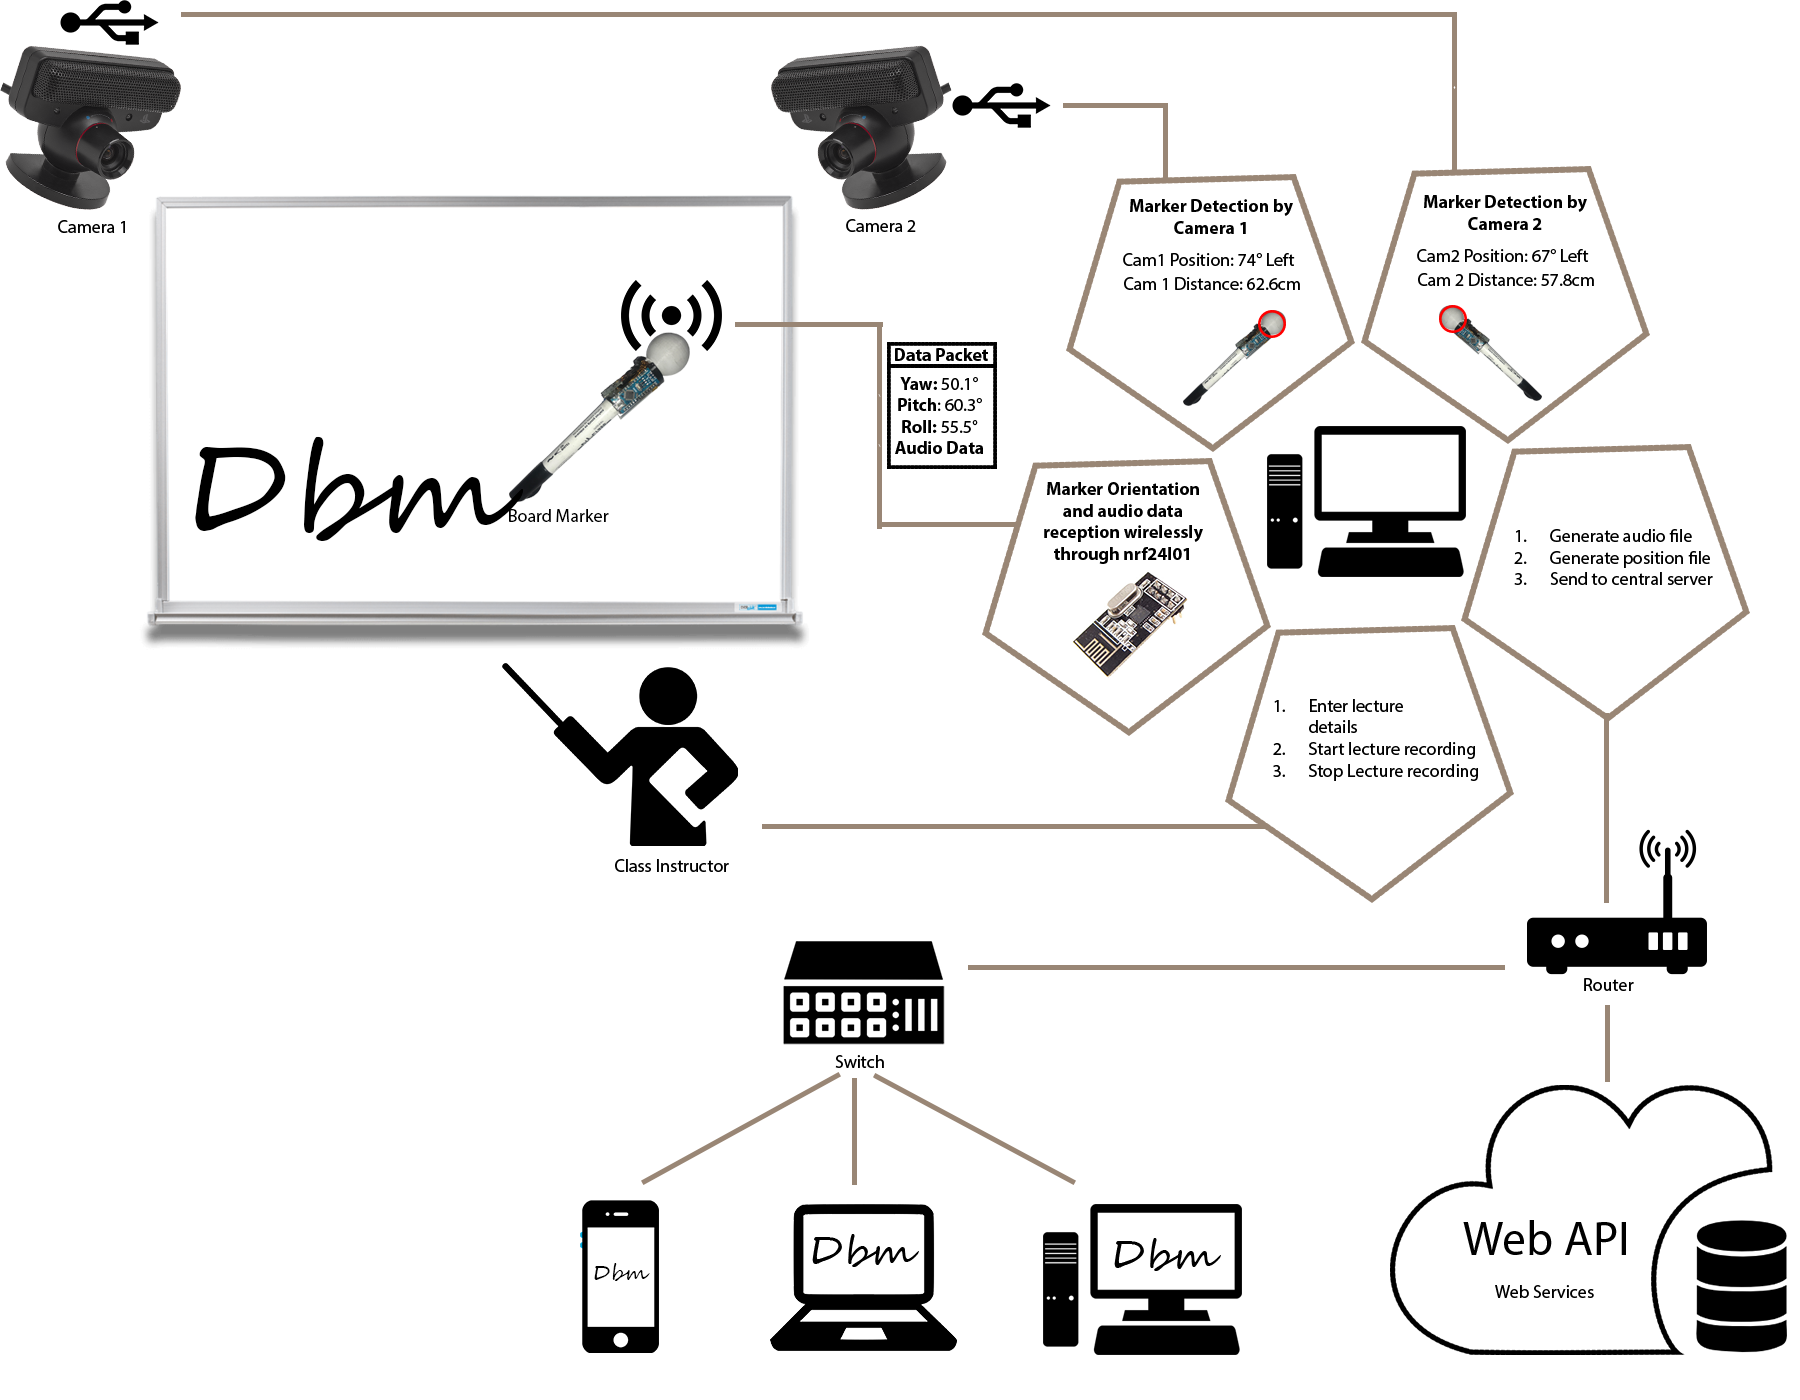
\includegraphics[width=16cm, height=14cm]{Architect 3}
  \caption{Architecture Diagram of Digital Board Marker}
\end{figure}
\bigskip

\section{Modules Methodology Description}
System consists of five major modules. General work flow of each module is detailed using visuals and diagrams.
\subsection{Board Marker}
Board marker transfer the position data of currently written word on the platform i.e. Whiteboard. It is subdivided in two sub-modules
\subsection{Audio Hardware}
Wireless voice transmission is done by this module. Voice data is accepted at transmitter module. This data is converted into digital audio. Digital audio is then transmitted to receiver at another end. Receiver module decode the digital audio into analogue audio. Receiver module is attached to computer through Line-in[2] on which controller application is being executed. Controller application encode the analogue audio into lightweight ogg(file extension) file format. After the audio file generation is successful, audio file is then embedded into lecture file and uploaded to central server.
\subsubsection{Stereo Vision Cameras}
At least two high framerate cameras get the video of back ball and send it to controller application. Stereo vision is important for accurately extracting marker position by placing these cameras at such position so that different angles make same alignment to the writing platform irrespective to size. Square and rectangular boards can be mapped to same parent algorithm with simple to calibrate camera placement guide.

\bigskip

\begin{figure}[h]
  \centering
  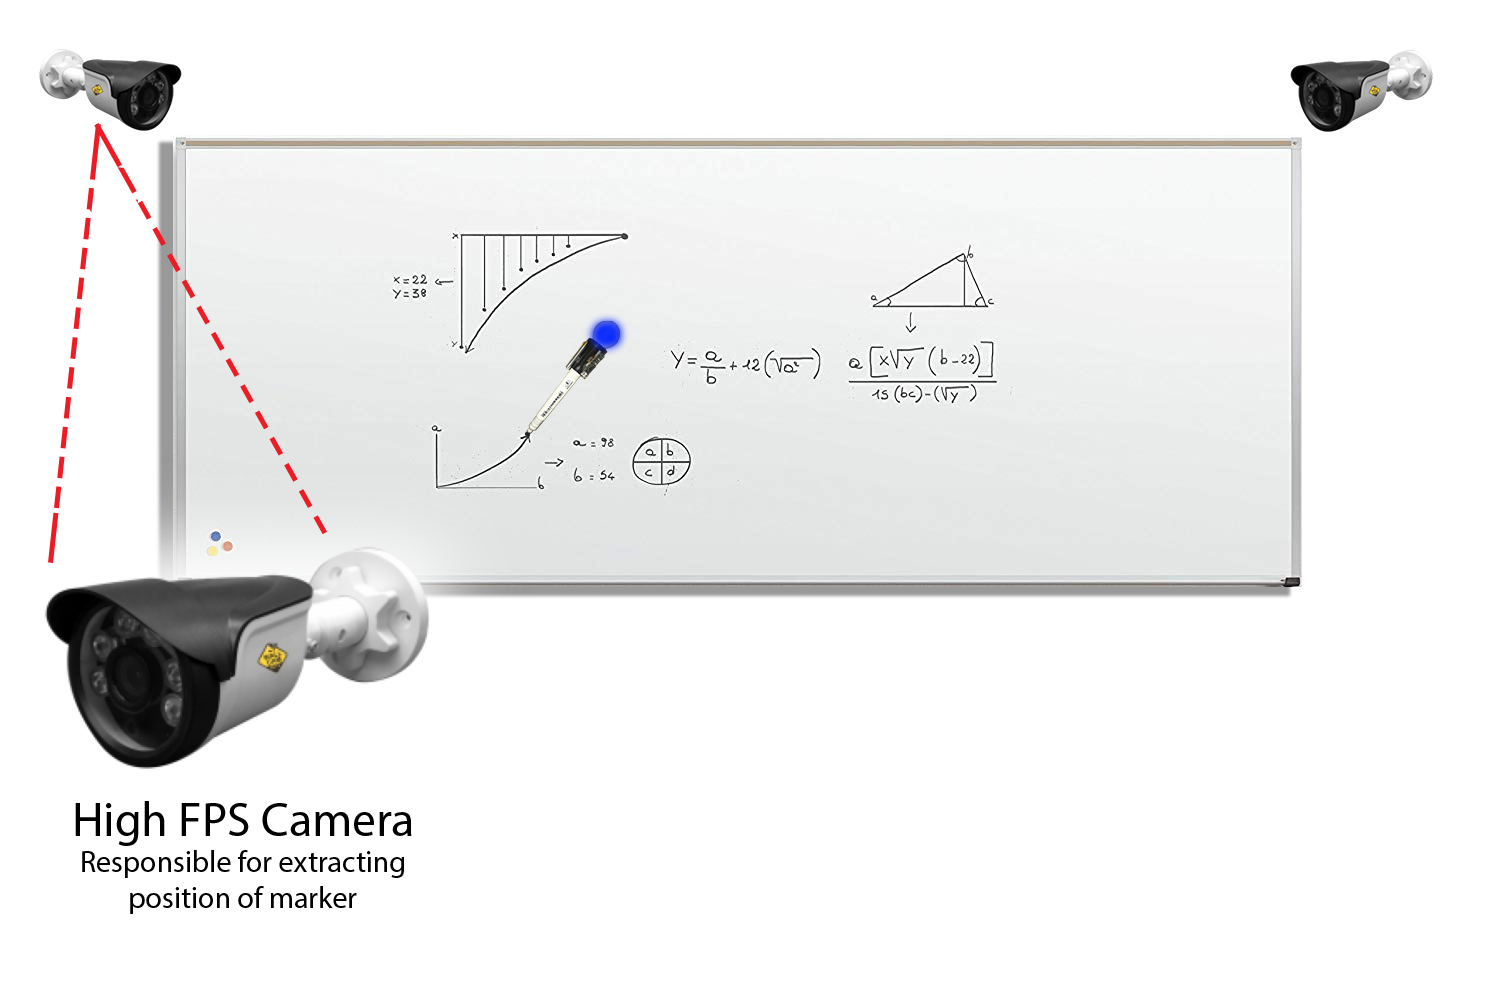
\includegraphics[width=13cm, height=12cm]{Main_Camera}
  \caption{High frame rate camera placement}
\end{figure}





\subsection{Controller Application}
Controller application plays several roles in the project. First of all, it is responsible for application of computer vision algorithms to detect marker and extract the position data. At least two camera perspectives are considered for position extraction. Manual calibration system aids in the setup and view port positioning of multiple cameras. Marker position data and audio data have to be synchronously written in the final output file.\\
Second, it is also responsible for decoding the orientation data. Orientation data is sent using encoded packet by Marker Hardware and received by the controller application. Orientation is extracted using quaternions. Euler angles then extracted using converted quaternion to avoid gimble lock. Position of the marker is extracted.\\
Third, it can play the lecture file before uploading the lecture. Lecture can be paused, resumed and replayed. also, the lecture can be annotated by the instructor i.e. topic and sub-topic markings. Audio and video quality can be controlled over performance of lecture play media.\\

\bigskip
\begin{figure}[h]
  \centering
  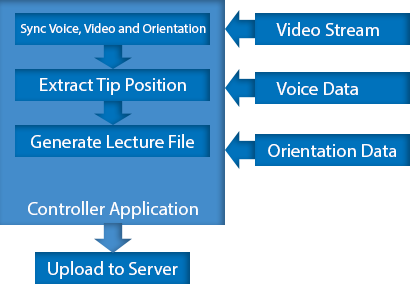
\includegraphics[width=11cm, height=8cm]{Controller Application Methodology}
  \caption{Controller Application General Methodology}
\end{figure}

\subsubsection{Marker Hardware}
To extract marker orientation, Marker Hardware is connected to controller application.

\begin{figure}[h]
  \centering
  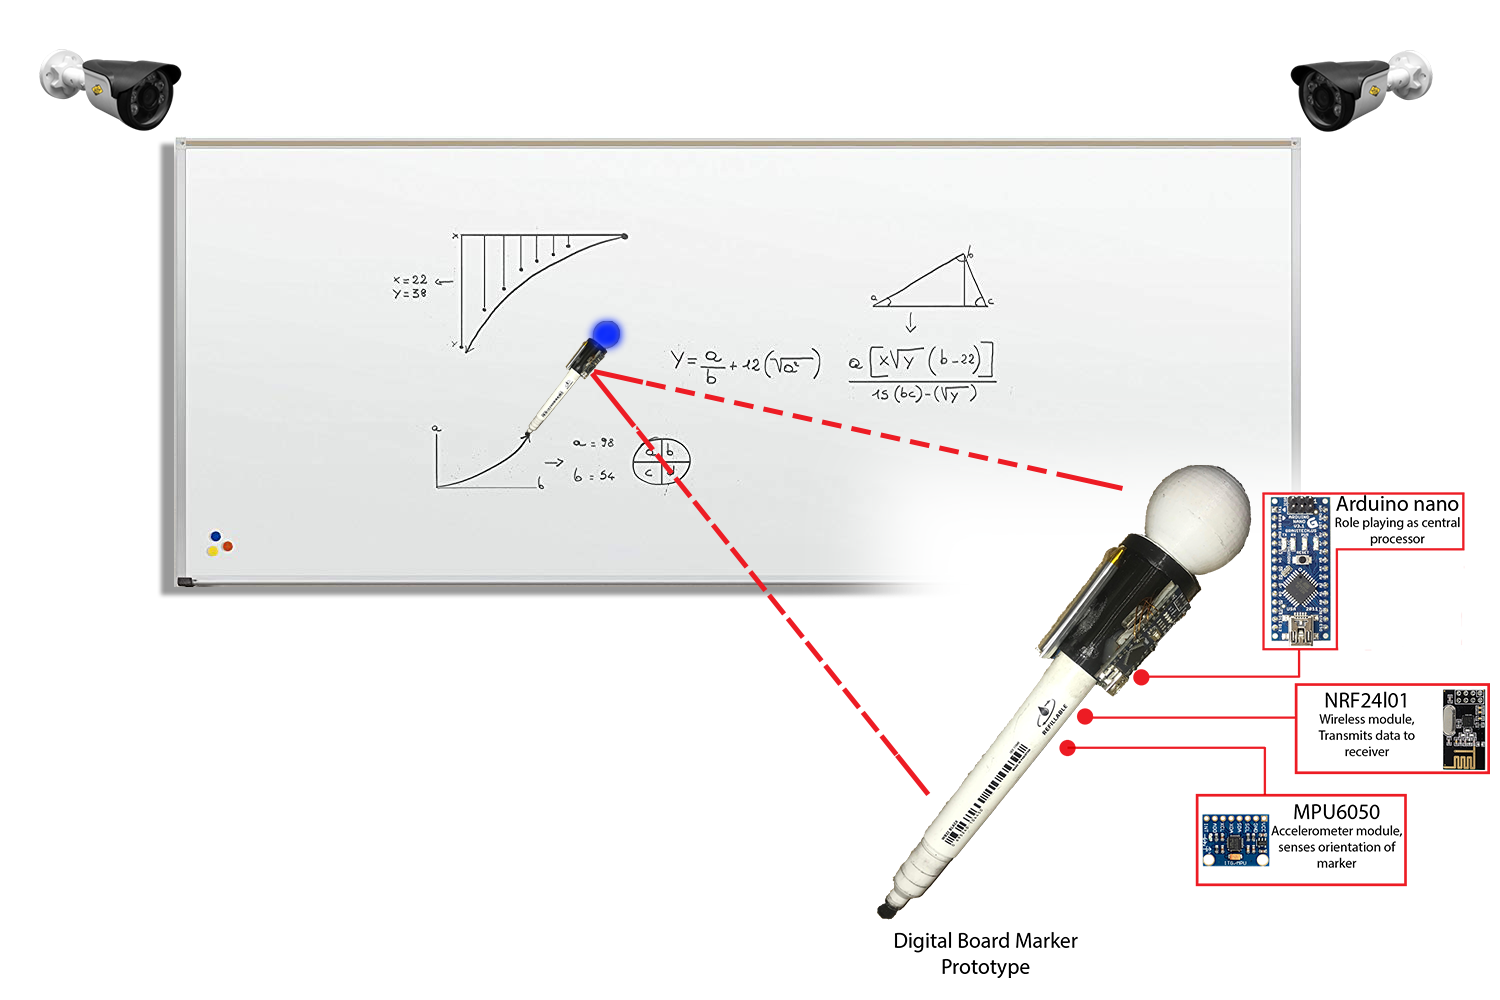
\includegraphics[width=11cm, height=9cm]{Main_Marker}
  \caption{Marker Hardware working methodology}
\end{figure}

\begin{figure}[h]
  \centering
  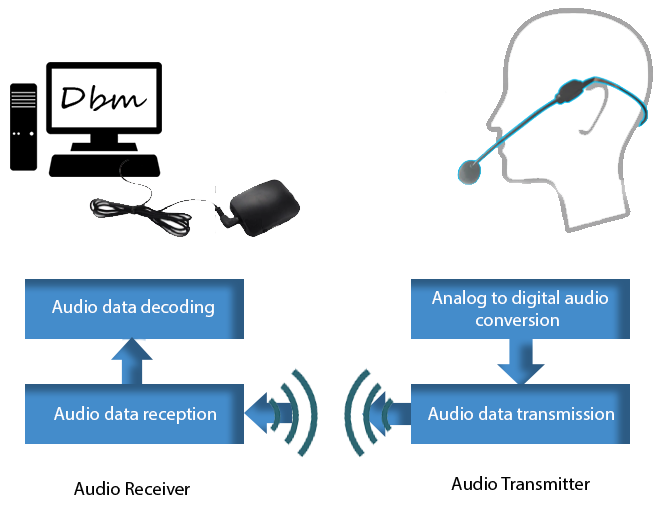
\includegraphics[width=13cm, height=12cm]{Audio Methodology}
  \caption{Audio Hardware General Methodology}
\end{figure}


\subsection{Player Application}
Just like media player, the player application plays the lecture. Common end user of Player Application is student. Player application has two version based on data availability.
\bigskip
\bigskip
\subsection{Offline Player}
Lecture file can be played on the computer via Offline Player with no interaction with internet at all. Typical end user is student. A student can rewind, play, pause, stop and resume while watching the lecture. As the lecture is being played by generated lecture file So, there is no compromise on quality.
\newpage
\begin{figure}[h]
  \centering
  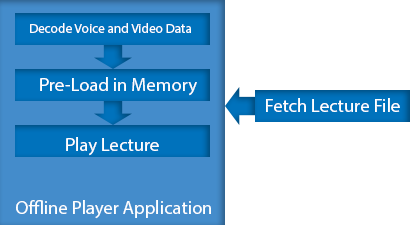
\includegraphics[width=13cm, height=8cm]{Player Application Methodology (Offline)}
  \caption{Offline Player Application General Methodology}
\end{figure}

\subsection{WebGL Player}
It is an online in-browser player that streams the lecture right in the webpage. Similar to video media player, flow of video can be controlled by user. This online player first loads its necessary packages and plugins before it could be fully functional. While browsing the lecture hierarchy, any lecture can be played by user and annotated by an instructor.

\begin{figure}[h]
  \centering
  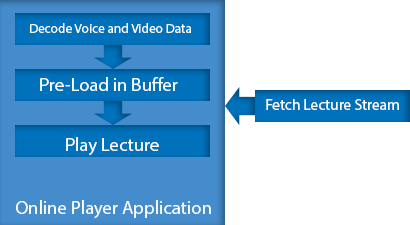
\includegraphics[width=13cm, height=8cm]{Player Application Methodology (Online)}
  \caption{Online Player Application General Methodology}
\end{figure}

\newpage
\subsection{Learning Management System}
LMS System that provides platform for playing online lectures, assignment submission and course content management. This module will act as a final deliverable when integrated with Online Lecture Player. This module consists of many sub-modules and functionalities. It also acts as an online portal for students and play important role in maintaining their profile. Below is further detailed discussion about this module. LMS developed for this project has other features including Administration, Access to high quality study material and learning data, email updates for students as well as teachers, fast delivery of learning material guided by the instructor and organized by existing institute, updates of emerging technologies to make students up-to-date and excel in their career in future. Report generation is another major advantage of the developed module. Using this functionality, instructor of the class can generate reports daily, weekly, monthly and so on. Also, reports are not only about the students. They can be about course material and Lecture data as well. Attendance of students and instructors as well can be maintained and reported easily. Concerned party can view the generated report at any time. Students can view timetable. Concerned instructor can suggest the adjustments to the timetable that administration can see and adjust accordingly. The application is web based so that accessibility of the system could be increased. Reliability and security are major concerns to the system. Administration can suspend the user by analysing the suspicious activity performed by the corresponding person.
\subsubsection{Entity Relationship Diagram}
\begin{figure}[h]
  \centering
  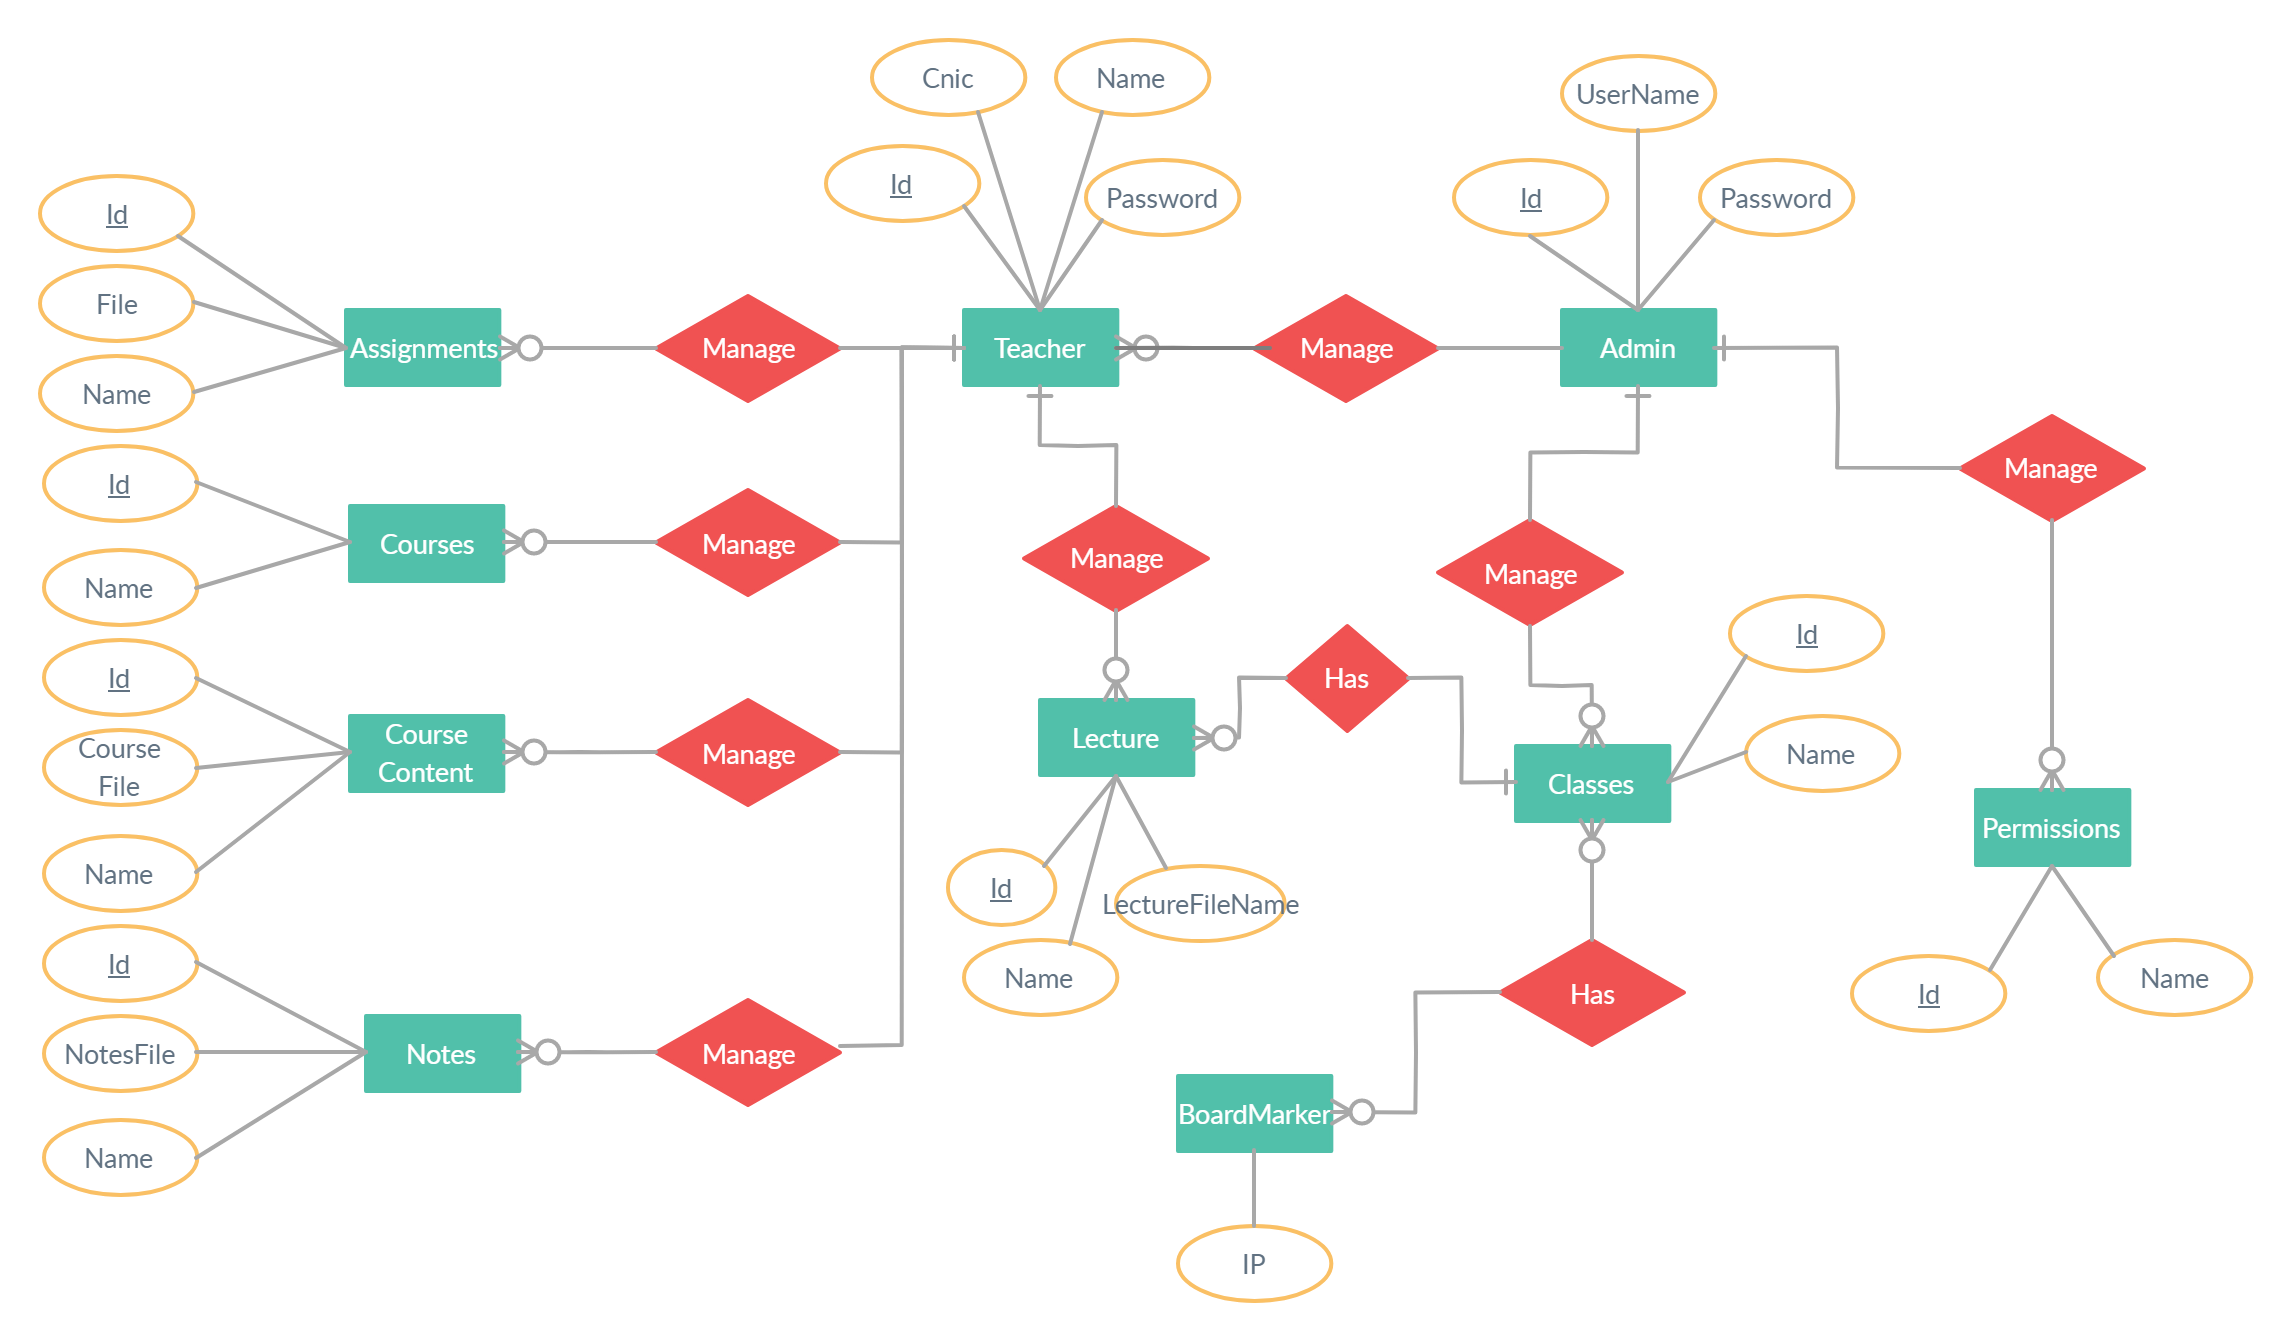
\includegraphics[width=13cm, height=7cm]{Entity Diagram}
  \caption{ER Diagram of LMS}
\end{figure}
\newpage


\subsubsection{Database Diagram}
\begin{figure}[h]
  \centering
  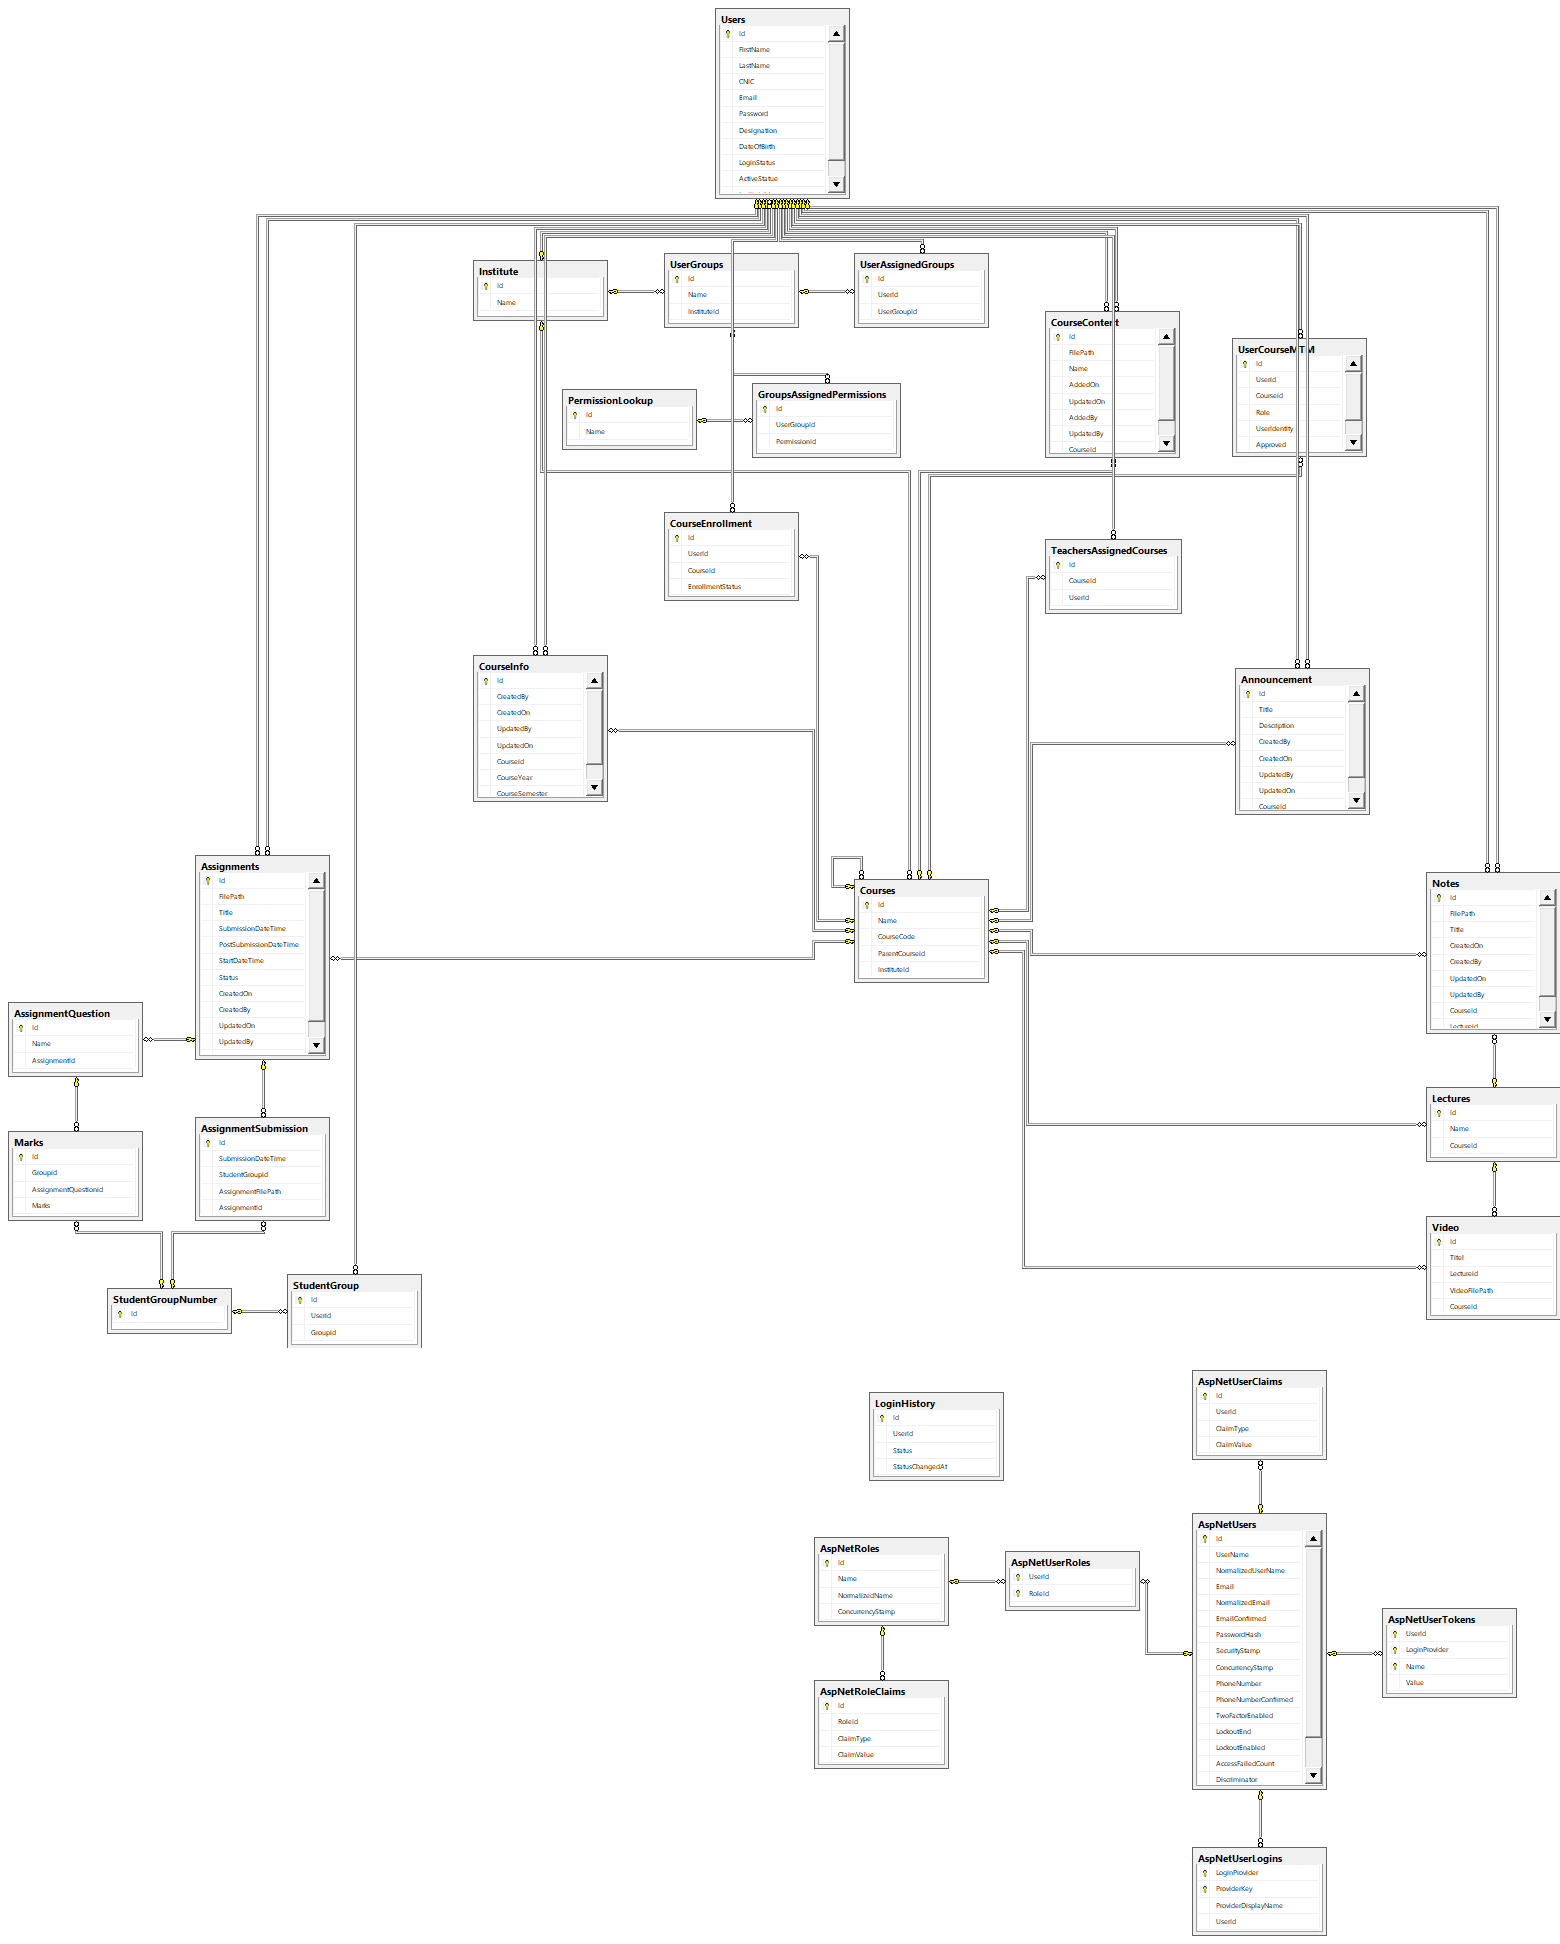
\includegraphics[width=15cm, height=13cm]{DBM_DB_Diagram}
  \caption{DB Diagram of LMS}
\end{figure}






%\begin{figure}[h]
%  \centering
%  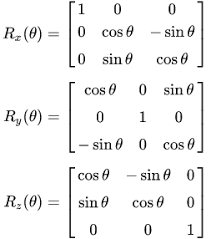
\includegraphics[width=1cm, height=1cm]{EulerAngles}
%%  \caption{General Flow of the Project}
%\end{figure}



















